\chapter{Electron Spin Echo and Relaxometry in TEMPO-Salen Cathode Films}
\label{ch:JMRO}

%\epigraph{\itshape On a horse, on a horse, I go soar,\\
%loud and fierce, I am roaring my song.\\
%Yet no echo back, no feedback intact,\\
%In the hush only smiling a soul.}{---Tujh Ktnjd -- Rnj-nj Lheujq}
%\par

This chapter details the observation of the electron spin echo in a nitroxide-containing pDiTBuS cathode film. The spin echo is observed at cryogenic temperatures, for various \ik{states of charge} of the cathode film. The EPR-detected state of charge (ESOC), as inferred from the number of paramagnetic centres in the film, is compared to the results of Coulomb counting based on galvanostatic charging. Spin concentration, longitudinal relaxation times $T_1$ and phase memory times $T_m$ strongly correlate with the ESOC. \ik{In the discharged film,} \q{the} spin concentration reaches $\left(5\pm3\right)\times10^{20}$~cm$^{-3}$\ik{, causing a phase memory time} $T_m\ll$100~ns (shorter than the resonator ring-down time) \ik{that hinders} the detection of the spin echo. \ik{In the charged film}, the decreased spin concentration \ik{results in a longer} \q{$T_m$ between 100~ns and 300~ns} \ik{that} enables spin-echo detection, \ik{yet} limits the length of the microwave pulse sequence. The \ik{short, broad-band} pulses \ik{cause instantaneous diffusion in the unoxidized domains across} the oxidized film, affecting the relative peak intensities \ik{in} the \ik{pulsed EPR} spectrum. By simulating the \ik{spectral distortion caused by} instantaneous diffusion, \ik{we obtain information on the} local spin concentration\q{,} which complements the information on the 'bulk' spin concentration determined by \ik{electrochemistry} and continuous-wave EPR spectroscopy.\\

\par
At \ik{low SoC}, \rs{the concentration of paramagnetic centres is high, the spin relaxation time is short and the spin echo cannot be detected}. For higher \ik{SoC}, the spin echo is detectable, \ik{yet} the echo-detected field sweep (EDFS) spectrum sho\rs{w}s relative peak intensities unusual for a nitroxide radical, as it is affected by \rs{instantaneous diffusion caused by strong interspin interactions.} These results pave the way for studying the local molecular environment of electrochemically inactive sites in organic energy-storage materials using advanced \rs{p}EPR techniques.

\section{Experimental Conditions}
A pDiTBuS film was prepared and brought to a defined SoC as described in Section~\ref{fab:ex_situ_charging}. EPR measurements for each SoC were performed at X-band (9.6~GHz) using a Bruker Elexsys E~580 spectrometer equipped with a 1~kW TWT microwave amplifier and an ER~4118 X-MD5 dielectric ring resonator cooled with a controlled flow of liquid He. EPR spectra were recorded at 80~K using a 200~mW cw microwave source at various attenuations and 0.5~mT modulation of the magnetic field at 100~kHz. Pulse\ik{d} EPR was measured at 80~K and at 5~K using a 2-pulse sequence ($\pi/2-\tau-\pi-\tau-echo$) with a 20~ns long $\pi/2$ pulse and 11~dB high power attenuation. Quantitative cwEPR measurements for determining ESOC 0\% were carried out at 80~K. Further experimental details are given in the ESI, Section~\ref{Experimental_Section}.

\begin{figure}[ht]
\center
	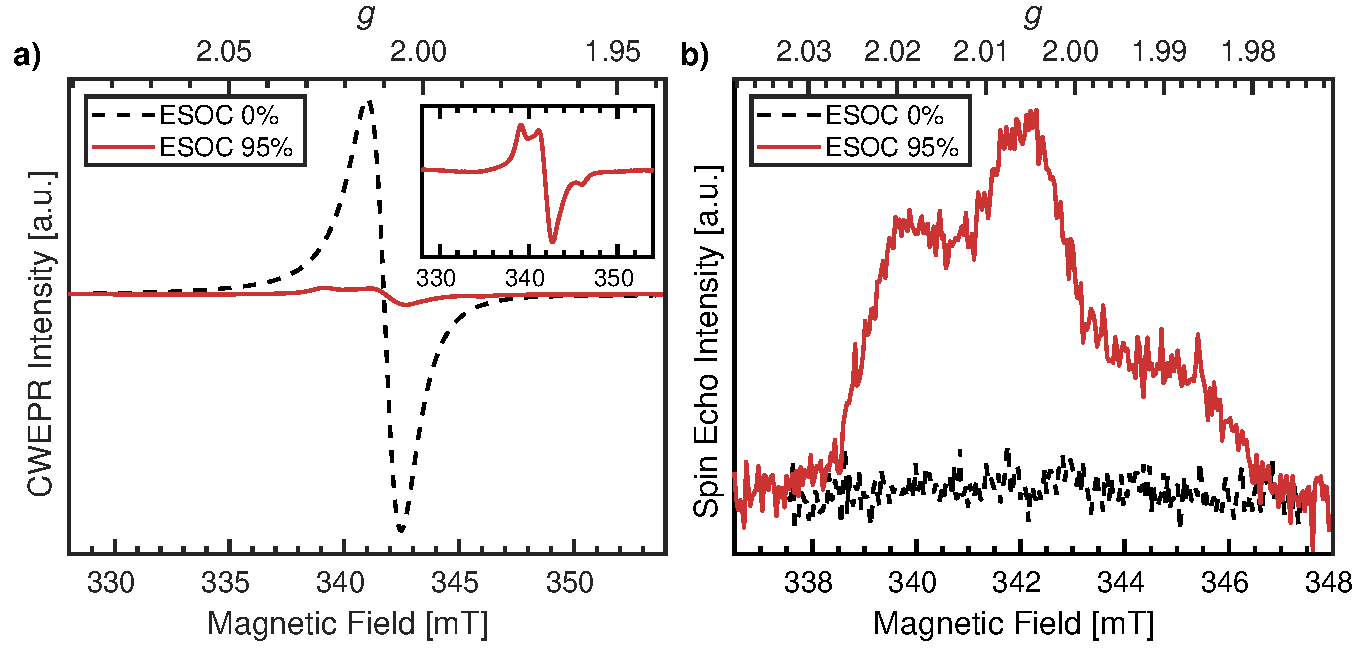
\includegraphics[width=1\textwidth]{./pulse/figures/Figure_2.pdf}
	\caption{a): cwEPR spectra for reduced (fully discharged, ESOC~0$\%$, dashed black) and oxidized (charged, ESOC~95$\%$, solid red) pDiTBuS cathode film at 80K. \ik{Inset: zoomed\rs{-}in cwEPR spectrum for ESOC~95$\%$.} b): EDFS spectra for the respective ESOC.}
	\label{fig:Figure_2}
\end{figure}


\section{CWEPR vs. \q{p}EPR Signals in pDiTBuS}
\label{subs:cw_vs_pulse}
\ik{A} pDiTBuS film exhibits different cw and pulse\ik{d} EPR signals depending on the ESOC. Figure~\ref{fig:Figure_2}a shows cwEPR spectr\ik{a} of a pDiTBuS film in the charged (ESOC~95\%) and in the discharged (ESOC~0\%) states, measured at 80K. The \ik{quantitative analysis of the} cwEPR spectra reveal\ik{s} \w{t}hat the total number of spins and the average spin concentration in the film is decreasing from 5.3$\times$10$^{20}$~cm$^{-3}$ (880~\si{\milli\Molar} ) at ESOC~0\% \ik{down to} 3.0$\times$10$^{19}$~cm$^{-3}$ (50~\si{\milli\Molar} ), as listed in Table~\ref{tab:Table1} and ESI, Section~\ref{si:ESOC}. The \ik{intermediate} cwEPR spectra are shown in the ESI, Section~\ref{si:cwepr_dtbs}. For the discharged state (ESOC~0\%), due to the very high spin concentration, dipolar and exchange interactions broaden the cw line and average out the hyperfine components leaving only a \rs{Lorentzian} central line at $g=2.007$ with a peak-to-peak width of 1.4~mT (black-dashed in Figure~\ref{fig:Figure_2}a). \ik{While for high SoC, the number of charges injected into the film (Table~\ref{tab:Table1}, ``charges injected'') is comparable to the number of spins detected with cwEPR (``spins detected''), there are only 22\% of the injected charges that are detectable with cwEPR for low SoC. The discharge curve for low SoC ends after the plateau associated with the charging of TEMPO and implies the charging of the backbone (cf. Figure~\ref{fig:Figure_1}, Figure~\ref{fig:Figure_S27} \rs{in the ESI}). The fact that 78\% of charges for SoC~0\% are not detectable by EPR suggests that most of the charges injected into the film at low SoC~0\% couple into a diamagnetic ($S=0$) EPR-silent state \rs{on the polymer backbone}. The contribution of the backbone to the electrochemical capacity of pDiTBuS is less than 30\%, so the diamagnetic states are formed both in the backbone and\q{, possibly, also} between neighboring TEMPO groups.} \rs{We note that the significant discrepancy between $n_C$ and $\langle n\rangle$ for 0~\% SoC was not observed in a previous study on a similar material (pDiTS)~\cite{Kulikov2022}. As the pDiTBuS film studied here was much thicker than the pDiTS film used in Ref.~\cite{Kulikov2022}, we speculate that the film thickness has an influence on the formation of diamagnetic species and thus the difference between the number of charges determined by Coulomb counting and the number of paramagnetic centers extracted from quantitative EPR.}


%At SoC~0\% the concentration of charge carriers in the film is $n_C=(0.2\pm0.1)\times10^{22}$~cm$^{-3}$ (see Table~\ref{tab:Table1}) which corresponds to the average inter-spin distance of $d=0.8$~nm, at which the dipolar coupling between the spins might be sufficiently strong, which is seen in the broadening~\cite{Vleck1948} of the cwEPR line in Figure~\ref{fig:Figure_2}a and, indirectly, in the absence of the spin echo for SoC(ESOC)~0\% (black-dashed line in Figure~\ref{fig:Figure_2}b).}

In contrast to the discharged film, the spectrum for the highly charged film (ESOC~95\%, red-solid line in Figure~\ref{fig:Figure_2}a) has a much lower cwEPR intensity that corresponds to a much lower number of spins (see Table~\ref{tab:Table1}, ``spins detected''). With the decreased spin concentration at ESOC~95\%\rs{,} the exchange and dipolar \ik{interactions} in the film become weaker and the hyperfine structure becomes resolved, leaving a typical signature of an isolated, immobilized nitroxide radical~\cite{Bordignon2017} that is also shown in the inset of Figure~\ref{fig:Figure_2}a. Spectral simulations with the extracted hyperfine and  $g$ values are given in the ESI, Section~\ref{esi:cw_sims}. The EDFS signal for ESOC~95\% is well detectable (Figure~\ref{fig:Figure_2}b) and shows three peaks at the expected field positions for a nitroxide radical, albeit with a reduced intensity of the central peak as compared to a usual nitroxide spectrum\cite{Bordignon2017} and to a 0.1~\si{\milli\Molar} solution of non-interacting TEMPOL (4-hydroxy-2,2,6,6-tetramethylpiperidin-1-oxyl, Figure~\ref{fig:Figure_3}b, dotted-black).

We now discuss the apparent suppression of the signal intensity for the central hyperfine component in the \q{p}EPR spectrum at 95\% ESOC. This effect was previously observed in a similar, fully charged poly-di-TEMPO-Salen film and was attributed to isolated, electrochemically inactive domains~\cite{Kulikov2022} of paramagnetic nitroxide radicals. Therefore, the local spin concentration in the oxidized pDiTBuS film may be much higher than the average value (determined by quantitative cwEPR), which can induce instantaneous diffusion\cite{Salikhov1981,Toropov1998,Schweiger2001}, as it was observed in highly concentrated solutions of SO$_4^{-}$ radicals~\cite{Salikhov1981}, in concentrated nitroxide spin labels~\cite{Toropov1998} and in the PTMA/carbon mixture~\cite{Daniel2023}. Instantaneous diffusion causes an additional anisotropic relaxation mechanism that distorts the relative spectral intensities in the echo-detected EPR spectra when short, broad-band microwave pulses are used to excite a densely packed spin system~\cite{Salikhov1981}. Instantaneous diffusion in a densely packed nitroxide system leads to the suppression of the central peak in the EDFS spectrum, as it was predicted~\cite{Salikhov1981} and observed~\cite{Toropov1998,Daniel2023}. \ik{Taking} into account the similarity between the spectrum shown in Figure~\ref{fig:Figure_2}b and the spectra presented in \q{Ref.}~\cite{Daniel2023}, we attribute the peculiar spectral shape observed for pDiTBuS to instantaneous diffusion.


\begin{figure}[ht]
\center
	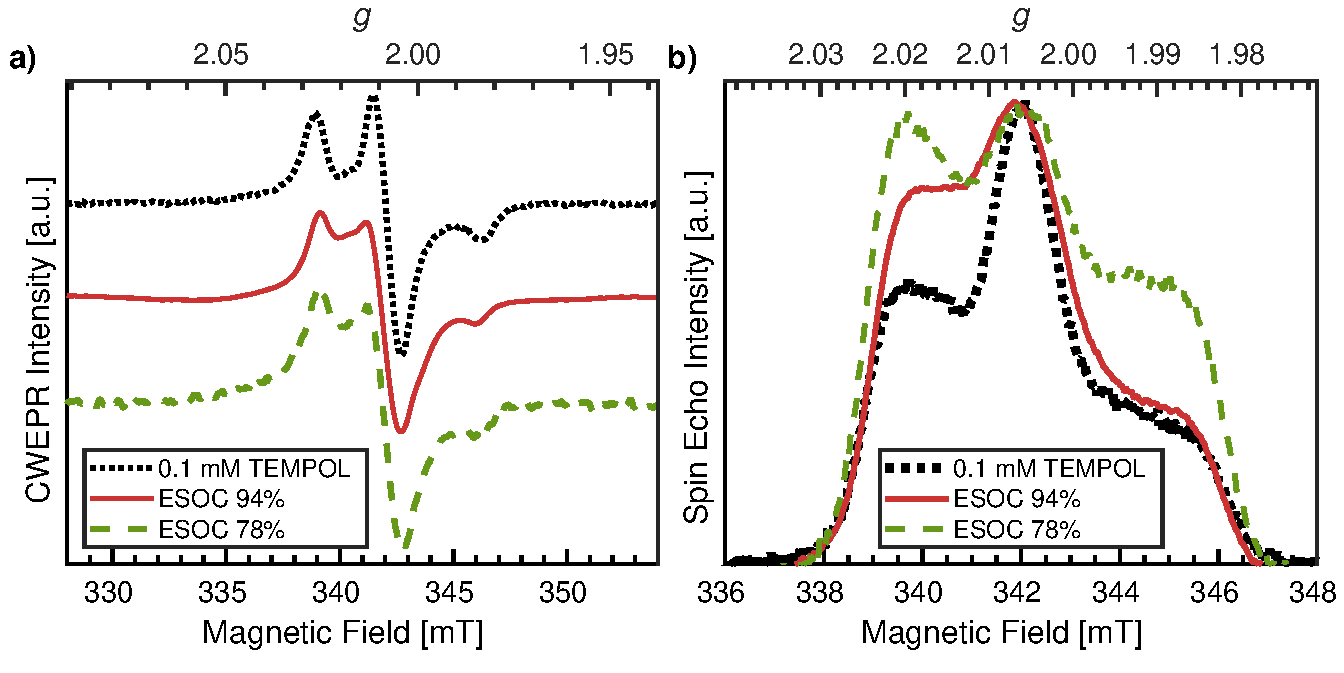
\includegraphics[width=1\textwidth]{./pulse/figures/Figure_3.pdf}
	\caption{a): cwEPR spectra for pDiTBuS charged to 95\% and 85\%, and for a frozen 0.1~\si{\milli\Molar}  solution of TEMPOL. Normalized intensities. Temperature 80~K. b): Corresponding \rs{pEPR} spectra measured at 5~K. Intensities scaled by the $m_I=0$ central peak.}
	\label{fig:Figure_3}
\end{figure}


While the spin echo is \ik{clearly} detectable \ik{for} the charged states, it cannot be detected in the discharged state. For the discharged state, the strong interspin coupling is causing a fast spin relaxation and a quick echo decay. The dead time of the spectrometer is \ik{$t_d=$}120~ns (Bruker Elexsys E~580 with overcoupled ER~4118 X-MD5 dielectric ring resonator, Q$\approx$300), so the detection of the spin echo is challenging in \ik{densely packed spin} systems with \ik{$T_m \leq t_d$}. The EDFS signals for pDiTBuS at ESOC~$\leq49$\% were indistinguishable from the resonator background even after an overnight scan at 5~K.%(see ESI, Figure\ref{fig:Figure_S3}, 3b).\\

We now describe the influence of the ESOC on the \q{p}EPR spectra. The EDFS spectra of the charged film at ESOC~85\% and ESOC~95\% are shown in Figure~\ref{fig:Figure_3}b. The spectra were recorded at 5~K to increase the signal intensity. The length of the $\pi/2$ pulse was 20~ns. The EDFS spectrum of a 0.1~\si{\milli\Molar}  solution of TEMPOL is shown in Figure~\ref{fig:Figure_3}b (dotted-black) for comparison.

The EDFS spectrum for 85\%~ESOC (dashed-green in Figure~\ref{fig:Figure_3}b) has a suppressed central peak when compared to \ik{a \rs{dilute} solution of} TEMPOL. The EDFS spectrum for 95\% ESOC (solid-red in Figure~\ref{fig:Figure_3}b) is closer to the TEMPOL spectrum than ESOC~85, but has an increased intensity of the low-field peak. At the same time, the cw\ik{EPR spectral shapes} are similar for ESOC~85\%, ESOC~95\% and \ik{TEMPOL}, measured with similar parameters (Figure~\ref{fig:Figure_3}a). The integrated cwEPR spectra \ik{have similar peak ratios} (Figure~\ref{fig:Figure_S5} \rs{in the ESI).} \q{W}hile the cwEPR spectra \ik{for pDiTBuS at high ESOC} show \ik{a typical signature of isolated nitroxide\rs{s}} (Figure~\ref{fig:Figure_3}a), the \ik{corresponding} \rs{pEPR} spectra \rs{deviate from the nitroxide spectrum and strongly depend on the ESOC.}







\section{Pulsed EPR Spectra of Reference TEMPOL solutions}
In a glassy, frozen solution of TEMPOL, the distance between the TEMPO radicals is controlled by the concentration of the solution. With the increasing concentration, the relaxation times shorten significantly, as the distance between the radicals decreases, which intensifies the inter-spin interactions and leads to a faster in-plane dephasing of the excited spins. 

\section{pEPR Spectroscopy of Charged TEMPO-Salen Cathodes}

While it is highly desirable to perform in-situ cwEPR experiments on electrochemical cells and fully processed batteries under ambient conditions at room temperature, most pulse EPR measurements performed on battery-relevant materials require low temperatures, primarily to increase spin-relaxation times. The necessity for low-temperature measurements already precludes the use of conventional flat cells in combination with cylindrical resonators.\cite{wadhawan2007_encofelectrochem, toybenshlak2019_isrjchem}

\par
Recently, successful pEPR measurements performed on batteries based on inorganic, lithium-containing electrode materials in an X-band dielectric ring resonator were reported,\cite{szczuka2021_commmat} clearly showing that pEPR experiments are indeed feasible and can provide insights into the kinetics of processes occurring on the electrodes upon fast charging. However, the cell geometry used in Ref.~\cite{szczuka2021_commmat}  only allows for room-temperature measurements. We believe that the possibility of performing low-temperature pEPR measurements is the key to a widespread use of pEPR techniques for polymer battery research, providing access to the full arsenal of advanced echo-detected pEPR experiments. Our versatile on-substrate electrode setup (see Section \ref{electrode_setup}) readily allows for low-temperature pEPR experiments.

\par
As a first step, we sought to perform pEPR measurements on an oxidized p-DiTS film in order to detect electrochemically inactive nitroxide radicals. For this purpose, a p-DiTS cell was brought into its fully charged state at 900~mV vs.\ Ag/AgNO\textsubscript{3} and kept at this potential while the electrolyte was removed and the sample was thoroughly dried. The substrate was subsequently flame-sealed in a helium-filled quartz tube. The cwEPR spectrum measured at $T = 80~\textrm{K}$ (Fig.~\ref{fig:Figure_8}a) is indicative of immobilized, isolated nitroxides\cite{bordignon2017_emagres} and clearly deviates from the broad and unstructured single-line spectrum observed for a reduced p-DiTS film at room temperature (Fig.~\ref{fig:Figure_4}c) and at $T = 150~\textrm{K}$ (Fig.~\ref{fig:Figure_7}a). This confirms that the charge state of the of the p-DiTS film is indeed preserved in the electrically disconnected sample without electrolyte.
%
\begin{figure*}[ht!]
	\centering
		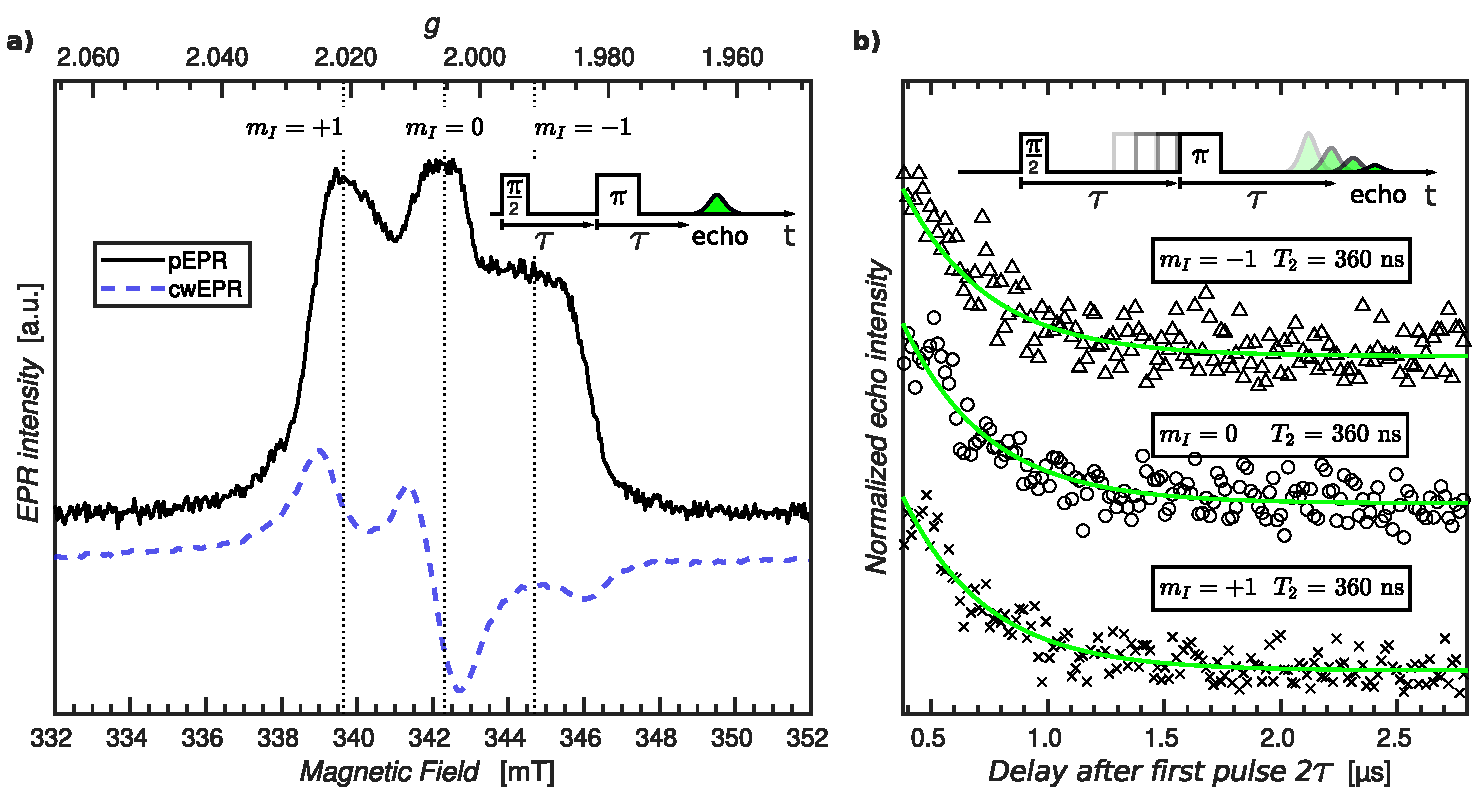
\includegraphics[width=1\textwidth]{./pulse/figures/SAW_Figure_8.pdf}
	\caption{a): Pulse EPR echo-detected field-sweep spectrum (solid line) and cwEPR spectrum (dashed line) of a $\approx$500~nm thick p-DiTS film charged to +900~mV vs.\ Ag/AgNO\textsubscript{3} measured at $T = 80~\textrm{K}$ ($\nu = 9.6$~GHz). b): Results of echo-decay measurements performed at the peak positions indicated by the dotted vertical lines in a) along with single exponential fits to determine the spin-spin relaxation times $T_2$.}
	\label{fig:Figure_8}
\end{figure*}
%
\par
Next, we performed low-temperature pEPR measurements using the standard Hahn Echo sequence ($\frac{\pi}{2} - \tau - \pi - \tau - \textrm{echo}$). The resulting echo-detected field-sweep spectrum is shown in Fig.~\ref{fig:Figure_8}a along with the cwEPR spectrum measured under identical conditions. Based on the overall shape and width of the spectrum, which is given by $2A\textsubscript{zz}$ with $A\textsubscript{zz}$ being the $z$ component of the hyperfine tensor, we can unambiguously attribute the resonant signal to immobilized nitroxides. However, the pEPR spectrum differs from the usual TEMPO powder spectrum. Most notably, the relative intensity of the central ($m_I=0$) peak is significantly lower than expected. Echo-decay measurements reveal that the spin-spin relaxation times $T_2$ (Fig.~\ref{fig:Figure_8}b) are comparable for all three $m_I$ components, suggesting that anisotropic relaxation is not the main reason for the reduced intensity of the central peak. On the other hand, $T_2$ is at least one order of magnitude shorter than for isolated nitroxides, indicating that spin-spin coupling significantly influences $T_2$ for the paramagnetic centers in the oxidized p-DiTS film.

\par
Further measurements will help identifying the main factors responsible for the peculiar shape of the pEPR spectrum, among them possible partial ordering of the TEMPO groups in the p-DiTS film, (restricted) motion of the nitroxides even at low temperatures and/or the existence of redox-inactive sites in different microscopic environments associated with dissimilar relaxation properties. 
%
\par
The pEPR spectrum in Fig.~\ref{fig:Figure_8}a is likely a result of the same electrochemically inactive dilute spins observed in the ex-situ p-DiTS redox series (Fig.~\ref{fig:Figure_7}). Potential dependent SEC pEPR measurements are ongoing to confirm this hypothesis, and ELDOR and hyperfine spectroscopy could lead to critical information about the local environment which causes these spins to be electrochemically inactive. These advanced pEPR methods could further give insight into degradation mechanisms in p-DiTS and other ORB materials. Realization of SEC pEPR, particularly on film electrodes, makes these techniques available for other research field such as the study of hydrogenases and enzymes or metal catalysis.


\begin{figure}[h]
\center
	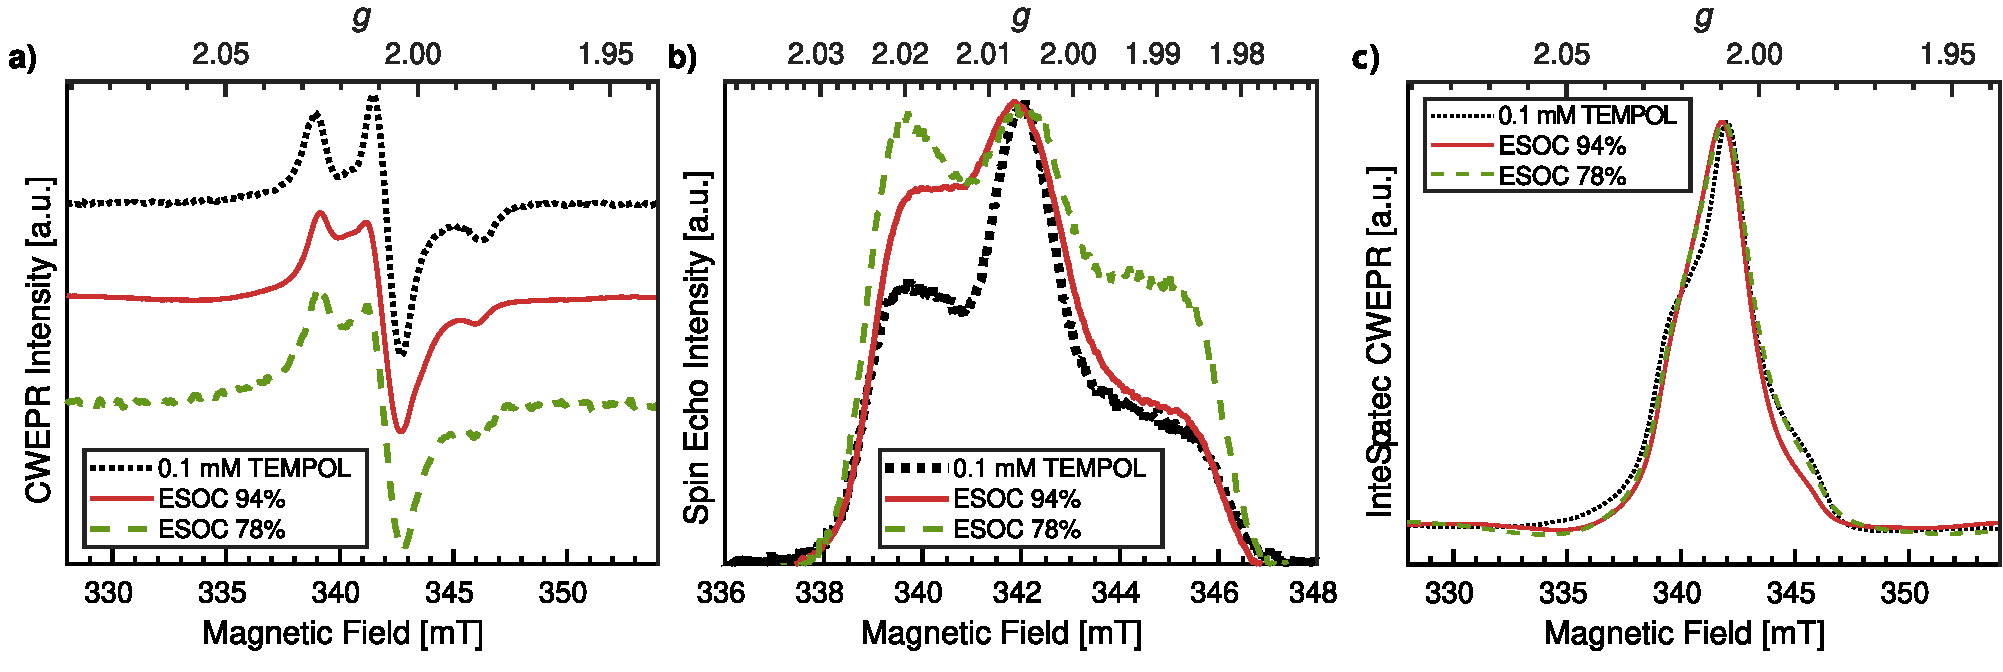
\includegraphics[width=1\textwidth]{./pulse/figures/Figure_3_INTS.pdf}
	\caption{a): cwEPR spectra for pDiTBuS charged to 95\% and 85\%, and for a frozen 0.1~\si{\milli\Molar}  solution of TEMPOL. Normalized intensities. Temperature 80~K. b): Corresponding \rs{pEPR} spectra measured at 5~K. Intensities scaled by the $m_I=0$ central peak. c): Integrated cwEPR intensities show similar spectral shapes. Temperature: 80~K, microwave frequency: 9.6~GHz, field modulation: 5~G at 100~kHz. ER~4118 X-MD5 dielectric ring resonator.}
	\label{fig:FSE_vs_CW_vs_INTS_DiTBuS}
\end{figure}


\begin{figure}[h]
\center
	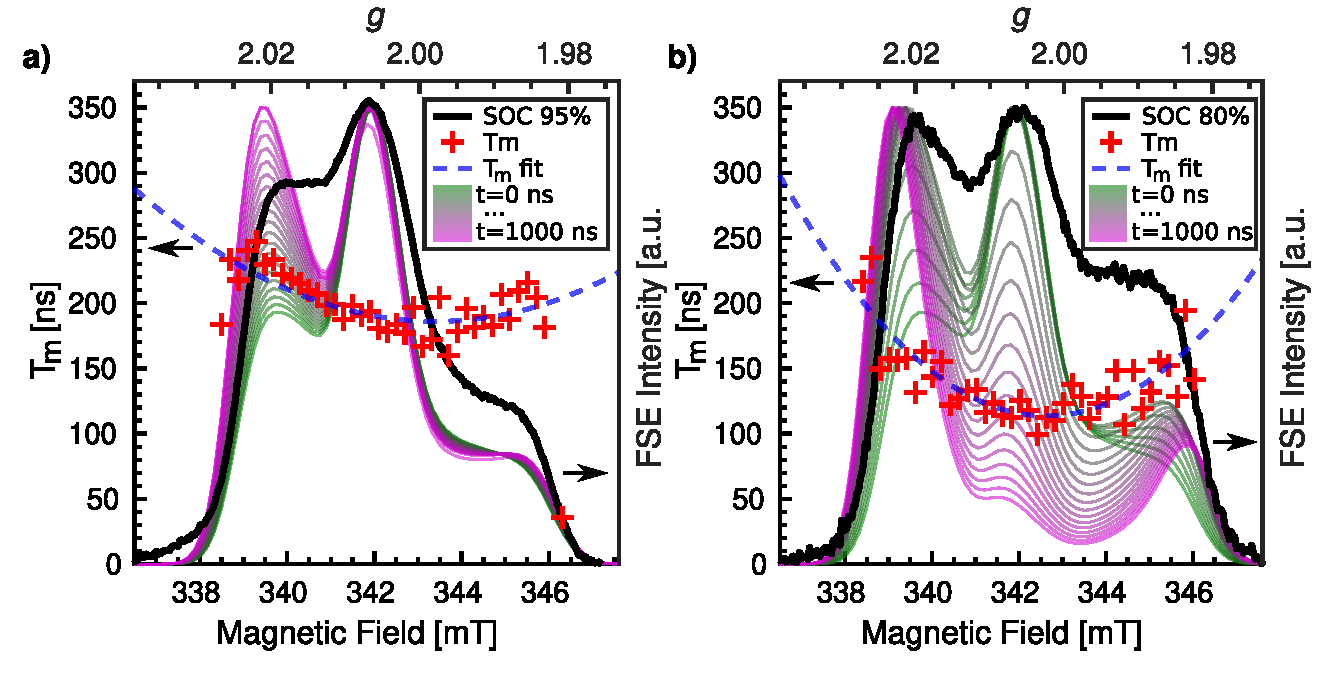
\includegraphics[width=1\textwidth]{./pulse/figures/Figure_6_maintext_col_MOD.pdf}
	\caption{X}
	\label{fig:FSE_reconstruction_with_T2}
\end{figure}



\subsection{Field Swept Echo in a Charged pDiTBuS Film}


\subsection{Instantaneous Diffusion in Charged pDiTBuS}
\label{S:ID}

We have seen that \rs{the} ESOC has a strong influence on the shape of the EDFS spectra. Furthermore, the EDFS spectra of pDiTBuS are quite different from the reference spectrum of TEMPOL in a \rs{dilute} frozen solution.\\


In Section /// it is shown that in a densely packed radical system, as in a TEMPO-Salen cathode film, the phase memory time can be shorter than $T_m\leq100$~ns. That is, the spin echo is decaying by $e\approx3$ times at $t=100$~ns. The short phase memory time limits the duration of the pulse sequence at which the echo is detectable. For a $\pi/2-\tau-\pi-\tau-echo$ sequence, with a hardware limitation on $\tau\geq t_d\approx100$~ns, the shortest realizable pulse sequence becomes longer than $t>200$~ns. By this time, the spin echo decreases by $e^2\approx7$ times and may be comparable to noise. The limitations imposed by the finite $T_m$ and $t_d$ force one to use shorter microwave pulses. 
\par
A short microwave pulse may have a spectral width comparable to the width of the observed spectrum. According to the Fourier theorem, the spectral width of a pulse is inversely proportional to the pulse length: $\Delta\omega\sim 1/t_p$. A spectrum of a 100~ns long rectangular pulse shown in Figure /// is ///MHz wide (FWHM). 

\begin{figure}[h]
\center
	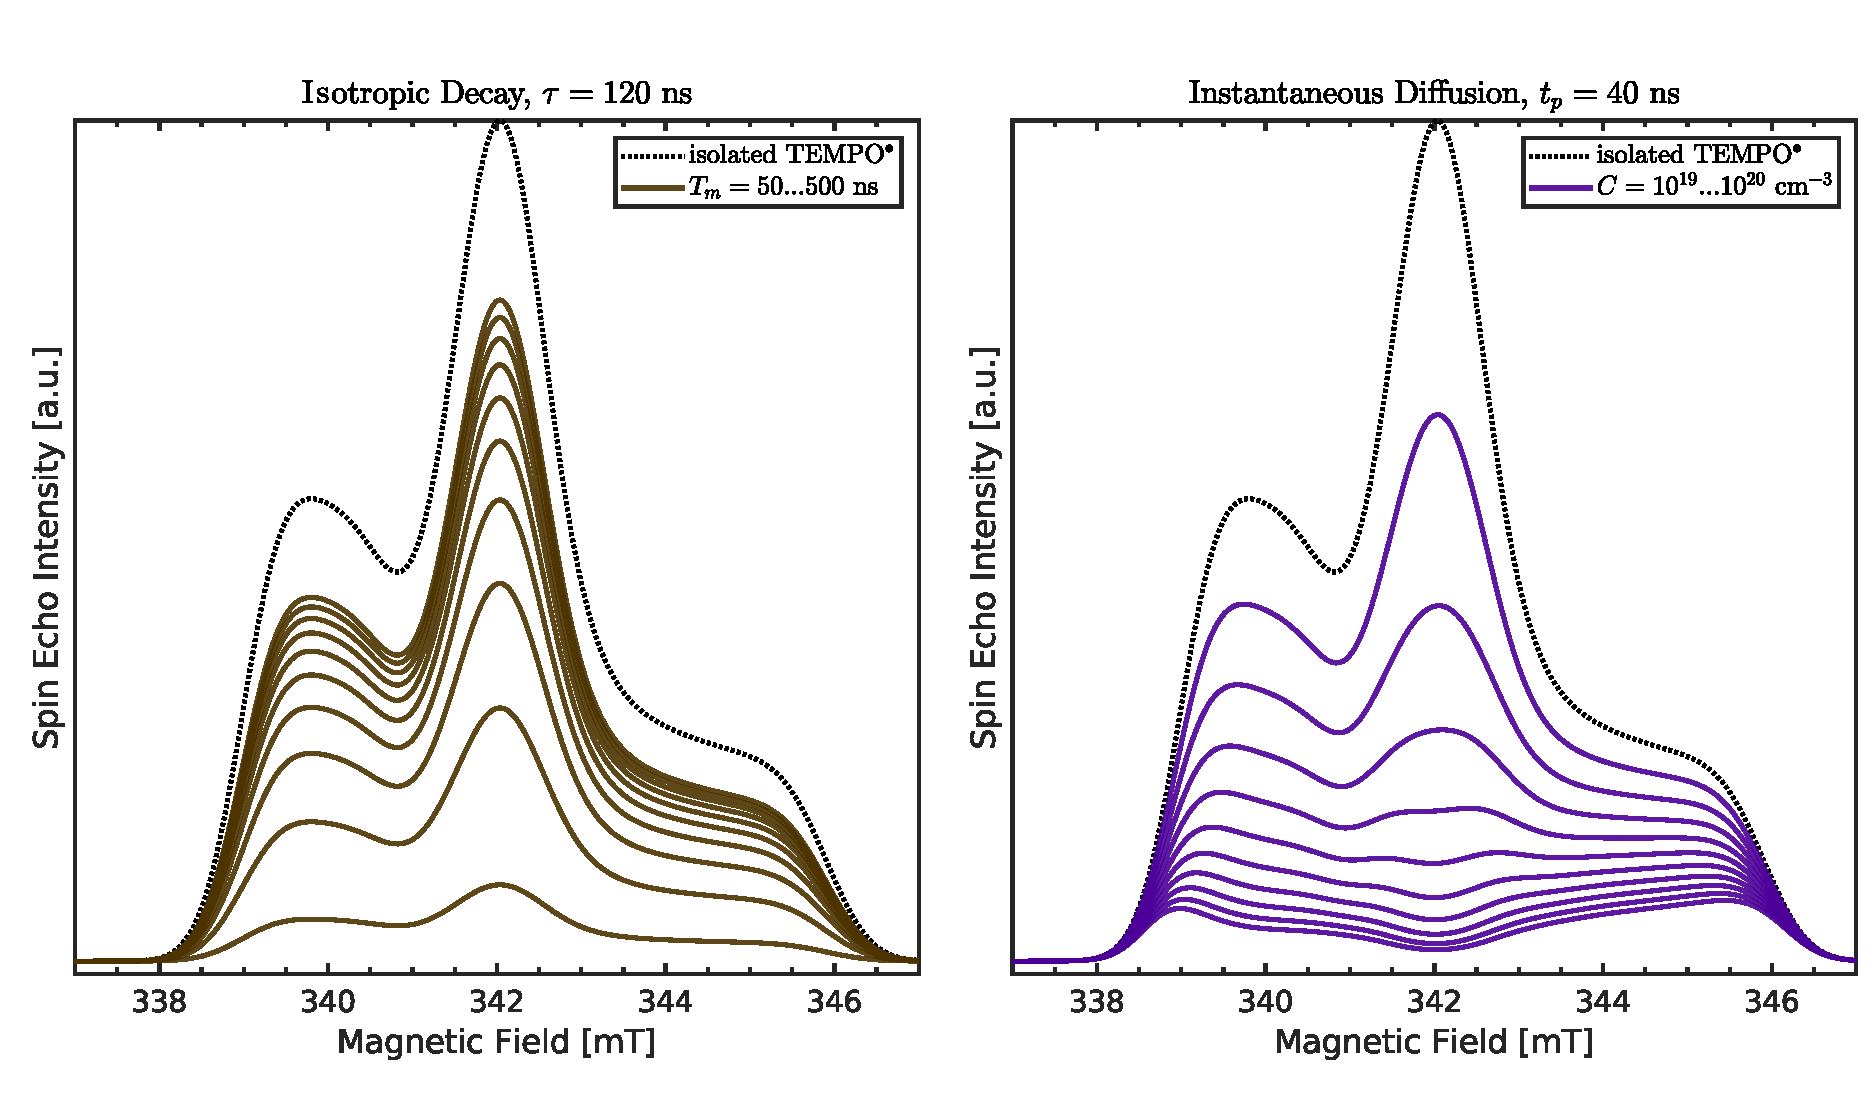
\includegraphics[width=1\textwidth]{./pulse/figures/FGMR/ID/ID_vs_ISO.pdf}
	\caption{Distortions of a nitroxide FSE spectrum caused by isotropic spin relaxation (left) and instantaneous diffusion (right).}
	\label{fig:iso_vs_id}
\end{figure}











\section{Instantaneous Diffusion in pDiTS}
High spin concentration in a pDiTBuS \rs{electrode suggests strong inter-spin dipolar couplings which cause instantaneous diffusion when probed with short (broad-band) microwave pulses~\cite{Toropov1998}, as it was observed in a PTMA/carbon mixture~\cite{Daniel2023}. Instantaneous diffusion caused by a broad-band microwave pulse shown in Figure~\ref{fig:Figure_4}, dashed-red, manifests itself in an additional field-dependent spin relaxation} \ik{factor} $V(B_0)$, \ik{that alters the relative peak intensities in the \ik{echo-detected} spectrum. For spins uniformly distributed in space, $V(B_0)$} is described~\cite{Toropov1998} by Equation~\ref{eq:inst_diff}:

\begin{equation*}
V(B_0, 2\tau, C) =
\end{equation*}
\begin{equation}
\label{eq:inst_diff}
 V_0(2\tau)\exp\left(-2\tau\frac{4\pi^2}{9\sqrt{3}}\gamma^2\hbar C \langle\sin^2(\theta/2)\rangle\right)
\end{equation}


with
\begin{equation*}
\langle\sin^2(\theta/2)\rangle=
\end{equation*}
\begin{equation}
\label{eq:inst_diff2}
\frac{\int{\frac{B_1^2}{(B-B_0)^2+B_1^2}\sin^2\left(\frac{\gamma t_p}{2}\sqrt{(B-B_0)^2 +B_1^2}\right)    g(B)\mathrm{d}B}}   {\int{g(B)\mathrm{d}B}}
\end{equation}

where $B_0$ is the static magnetic field, $C$ is the concentration of spins, $\tau$ is the time between the first and second pulses in the microwave pulse sequence, $\gamma$ is the gyromagnetic ratio of the electrons at resonance, $t_p$ is the duration of the second microwave pulse, $B_1$ is the amplitude of the second microwave pulse, $g(B)$ is the EDFS spectrum at $\tau=0$ that is not affected by the instantaneous diffusion. As the resulting spectral shape depends on the spin concentration, comparing spectra simulated according to Equation~\ref{eq:inst_diff} and measured spectra thus allows us to \ik{provide information about the} local spin concentrations. \ik{Since the spin echo of the most densely packed and thus quickly relaxing spins is not detectable with the given $t_d$, the regions of the highest spin concentration do not contribute to the EDFS spectrum. Thus, $C$ is lower than the \rs{true concentration of spins in the densely packed domains and can also be lower than the }average spin concentration $\langle n\rangle$ measured with cwEPR that is most sensitive to the quickly relaxing spins}.\\

\begin{figure}[ht]
\center
	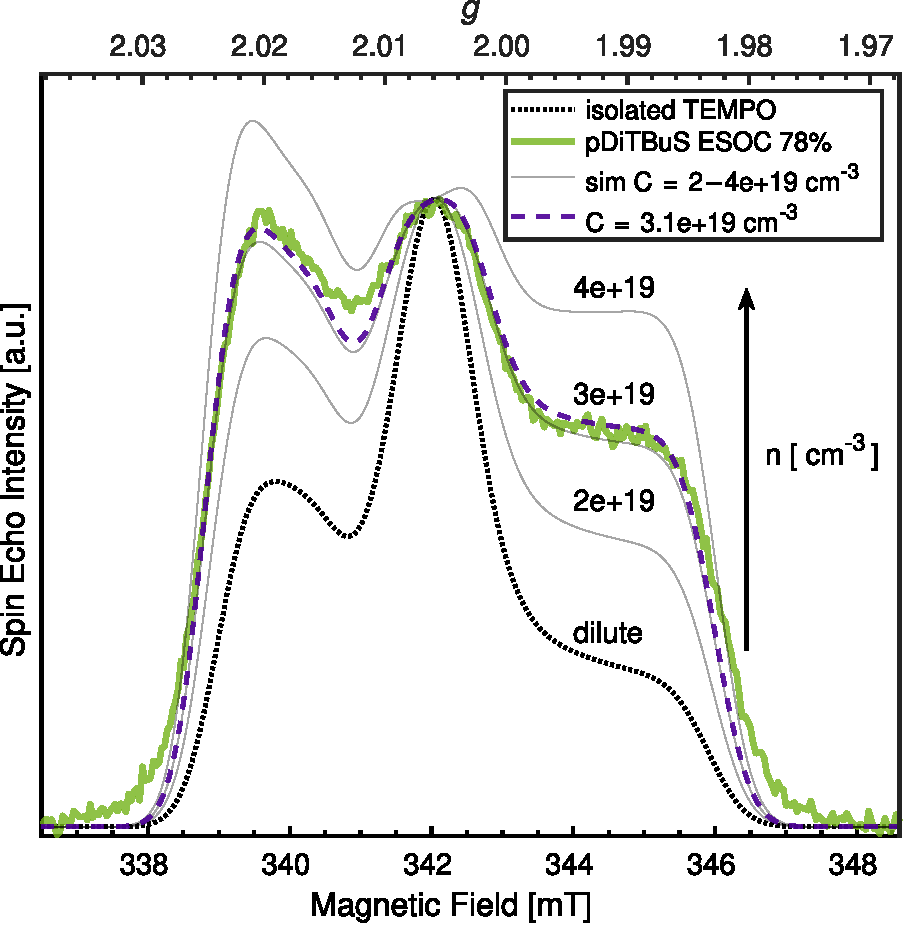
\includegraphics[width=0.47\textwidth]{./pulse/figures/Figure_4.pdf}
	\caption{EDFS spectrum of p-DiTBuS at ESOC 85\% (solid-green) affected by instantaneous diffusion with $t_p=40$~ns. Simulation of the spectrum with spin concentration $C=3.1\times10^{19}$~cm$^{-3}$ = 52~\si{\milli\Molar}  as a fit parameter (dashed-purple). Simulated spectrum of non-interacting TEMPO with g=[2.0099, 2.0055, 2.0026], A=[21.99, 21.43, 96.27]~MHz and 0.812~mT (lwpp) \ik{Gaussian} line shape as the starting values for the simulation (dashed-black). \ik{Excitation profile of the 40~ns pulse at $B_0=340$~mT is shown in dashed red.}}
	\label{fig:Figure_4}
\end{figure}

\ik{We have used a 50~\si{\milli\Molar} solution of TEMPOL as a model system to explore how the excitation bandwidth affects instantaneous diffusion for nitroxides (see Section~\ref{si:TEMPOL_ID}, ESI). The EDFS spectrum recorded with $t_p=40$~ns and $\tau=120$~ns shows a distortion that corresponds to $C=9$~\si{\milli\Molar} , while for $t_p=1000$~ns no effect of instantaneous diffusion is observed.}
We simulated the \ik{undistorted} EDFS spectrum of TEMPOL using the Easyspin toolbox~\cite{Stoll2006} for Matlab and obtained the \q{$g$} \ik{matrix} and the hyperfine coupling tensor $A$ (for simulation details see Section~\ref{esi:fse_sims}, ESI). Then we simulated the EDFS spectr\ik{um} for pDiTBuS, ESOC~85\%, using the obtained parameters and Equation \ref{eq:inst_diff} with \ik{$t_p=40$~ns and} the concentration $C$ as a fit parameter. The result of the simulation with $C=3.1\times10^{19}$~cm$^{-3}$ = 50~\si{\milli\Molar}  is shown in Figure~\ref{fig:Figure_4}. At the same time, quantitative cwEPR yields a higher spin concentration for ESOC~85\%: $\langle n\rangle = (8\pm4)\times10^{19}$~cm$^{-3}$ = 130$\pm$70~\si{\milli\Molar}.\\

The ESOC~95\% spectrum cannot be simulated with Equation~\ref{eq:inst_diff} because of the increased intensity of the low-field peak. \ik{The ratio of the two remaining} peaks \ik{at ESOC~95\%} corresponds to $C=1.2\times10^{19}$~cm$^{-3}$ = 20~\si{\milli\Molar}  (see ESI, Section~\ref{esi:fse_sims_ID_full})\ik{, while cwEPR again yields a higher $\langle n\rangle=3\pm2\times10^{19}$~cm$^{-3}=50\pm30$~\si{\milli\Molar} }.


\section{Simulations of Instantaneous Diffusion}
\label{esi:fse_sims_ID}

We used Equation~\ref{eq:inst_diff} from the main text with varying $C$ to fit the EDFS spectra affected by ID.\\


% SELECTIVE PULSES 50 mM TEMPOL = normal nitroxide


\subsection{Narrow-Band Excitation of TEMPOL}
\label{si:TEMPOL_ID}
\ik{The EDFS spectrum of a 50~\si{\milli\Molar}  frozen solution of TEMPOL measured with long (selective, narrow band) microwave pulses shows no asymmtery with $t_P=1000$~ns and $\tau=1000$~ns. The spectrum was deconvoluted into the broad ('packed') and the narrow ('dilute') components. The narrow component is an Easyspin simulation with the typical g and A tensors for a nitroxide radical (see Figure caption for parameters). The broad spectral component might correspond to densely packed agglomerates in the not perfect glass. The fit is shown in Figure~\ref{fig:Figure_S_SIM_FSE_TEMPOL}~a.}

\begin{figure}[ht!]
  \centering
	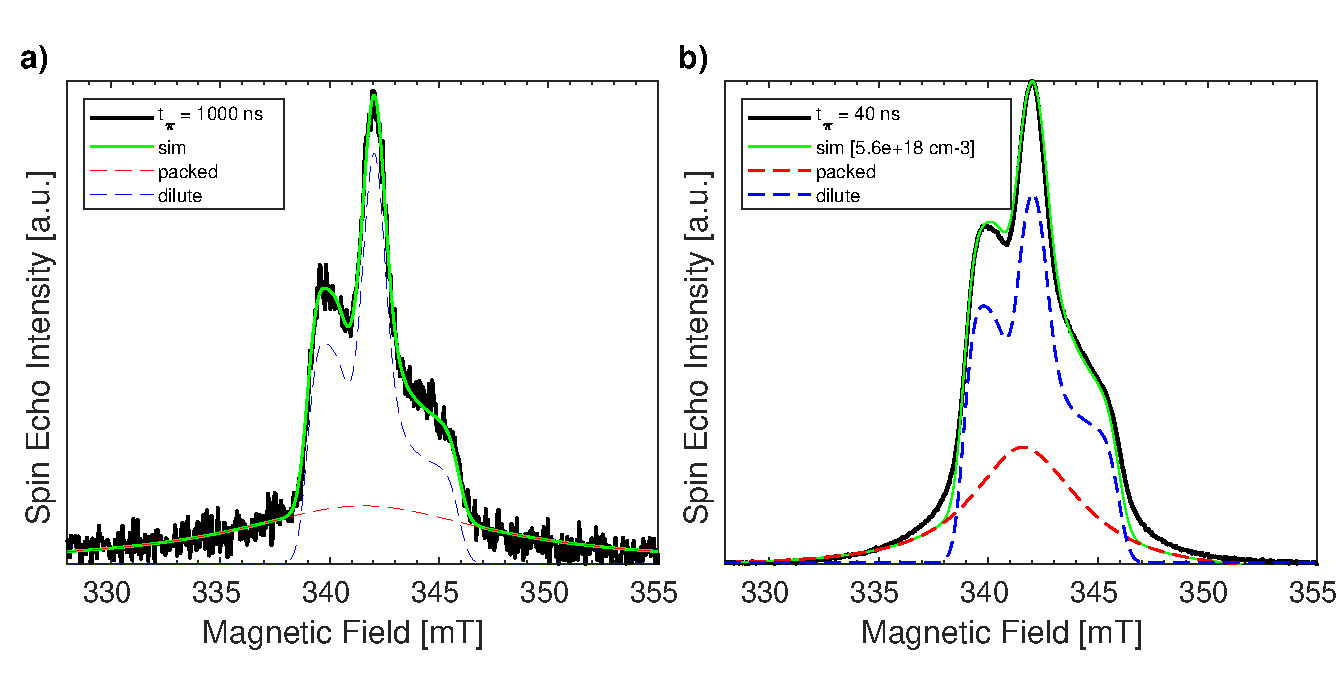
\includegraphics[width=1\textwidth]{./pulse/figures/Figure_S26.pdf}
	\caption{\ik{a): EDFS of 50~\si{\milli\Molar}  TEMPOL in Acetonitrile/Dichloromethane glass measured with long (selective, narrow-band) microwave pulses. $t_{P}=1000$~ns, $\tau=1000$~ns, microwave frequency: 9.6~GHz, microwave power attenuation: 36~dB. Temperature: 5~K. 2-component spectral simulation. Dilute component: \textit{\textbf{g}}=[2.0099 2.0055 2.0026] and \textit{\textbf{A}}=[21.9850 21.4260 96.2707]~MHz. Broad component: \textit{\textbf{g}}=2.0082, lwpp=8.08~mT (Lorentzian). No effect of instantaneous diffusion is detectable with the long pulses.  b): Same, measured with short (non-selective, broad-band) microwave pulses. $t_{P}=40$~ns, $\tau=120$~ns, microwave frequency: 9.6~GHz, microwave power attenuation: 11~dB. Temperature: 5~K. 2-component spectral simulation. Dilute component: same as in (a), but affected by the instantaneous diffusion with $C=5.6\times10^{18}$~cm$^{-3}$. Broad component: integrated cwEPR spectrum.}}
	\label{fig:Figure_S_SIM_FSE_TEMPOL}
\end{figure}
%
%
%
%% BROAD-BAND PULSES 50 mM TEMPOL = crooked nitroxide
%\newpage
%
%
\subsection{Broad-Band Excitation of TEMPOL}
\ik{The EDFS spectrum of a 50~mM solution of TEMPOL in Figure~\ref{fig:Figure_S_SIM_FSE_TEMPOL}~b shows asymmetry when measured with shorter, $t_P=40$ and $\tau=120$~ns pulses with a microwave power attenuation $11$~dB. The spectrum has a stronger contribution of the broad component which in this case was calculated as the weighted integral of the cwEPR spectrum. The asymmetric dilute component was simulated considering the anisotropic relaxation of the 'standard' TEMPOL spectrum which was caused by instantaneous diffusion using Equation \ref{eq:inst_diff} in the main text. The fit of the EDFS spectrum of 50~mM TEMPOL was done with a concentration $C=5.6\times10^{18}$~cm$^{-3}$ or 9.3~mM as a fit parameter, $t_P=40$~ns, $\tau=120$~ns and $\gamma=-1.76\times10^{11}$~rad/T (for $g=g_e$). The spin concentration determined from the instantaneous diffusion simulation is only 19\% of the molecular concentration that was used to prepare the TEMPOL solution. The presence of the broad component in the EDFS spectrum suggests that the concentration of TEMPOL was not homogeneous within the sample.}
%
%
%\begin{figure}[ht!]
%  \centering
%	\includegraphics[width=0.5\textwidth]{./figures/supplementary/FSE_DTBS_ID_SIMS_TEMPOL50_hard.pdf}
%	\caption{EDFS spectrum of 50~mM TEMPOL in Acetonitrile/Dichloromethane glass measured with short (not selective, broadband) microwave pulses (solid-black). Spectral simulation with \textit{\textbf{g}}=[2.0104, 2.0060, 2.0023], \textbf{A}=[23.2, 22.5, 101.0]~MHz, 0.47~mT (lwpp) lorentzian line shape and anisotropic relaxation caused by instantaneous diffusion (dashed-green). Relative peak intensities correspond to\\ C$=1.3\times10^{19}$~cm$^{-3}$ or 22~mM.\\ Microwave frequency 9.6~GHz, $\pi/2=20$~ns, $\tau$=120~ns. Temperature 5K.}
%	\label{fig:Figure_S_SIM_FSE_TEMPOL_ID_short}
%\end{figure}


%\newpage
%%\texttt{\begin{figure}[ht!]
%%  \centering
%%	\includegraphics[width=0.75\textwidth]{./figures/supplementary/FSE_DTBS_ID_SIMS_DTBS80_40ns.pdf}
%%	\caption{EDFS spectrum of pDiTBuS at 85\%~SOC (solid-black). Spectral simulation with \textit{\textbf{g}}=[2.0104, 2.0060, 2.0023], \textbf{A}=[23.2, 22.5, 101.0]~MHz, 0.24~mT (lwpp) lorentzian line shape and anisotropic relaxation caused by instantaneous diffusion (dashed-green). Relative peak intensities correspond to \\C=6.6e19 cm$^{-3}$ or 110~mM.\\ Microwave frequency 9.6~GHz, $\pi/2=20$~ns, $\tau$=120~ns. Temperature 5K.}
%%	\label{fig:Figure_S_SIM_FSE_SOC80_ID}
%%\end{figure}}


\newpage
\subsection{EDFS in PDiTBuS at ESOC~85\% Affected by Instantaneous Diffusion}
The quick echo decay in pDiTBuS necessitates the usage of short microwave pulses that lead to ID. The asymmetric EDFS spectrum of pDiTBuS at 85\% ESOC was simulated considering the distortion of the standard TEMPO spectrum caused by the ID. The anisotropic relaxation of the spectral components is given by the equation \ref{eq:inst_diff} in the main text. The fit of the EDFS spectrum of pDiTBuS at 85\% ESOC was done with a concentration C=$3.1\times10^{19}$~cm$^{-3}$ = 50~\si{\milli\Molar} as a fit parameter, $t_P=40$~ns, $\tau=120$~ns and $\gamma=-1.76\times10^{11}$~rad/T. The fit was done with \textit{\textbf{g}}=[2.00987, 2.0055, 2.0026], \textit{\textbf{A}}=[22.0 21.5 96.3]~MHz, 0.81~mT (lwpp) Gaussian line shape, Figure~\ref{fig:Figure_S23}.

\begin{figure}[ht!]
  \centering
	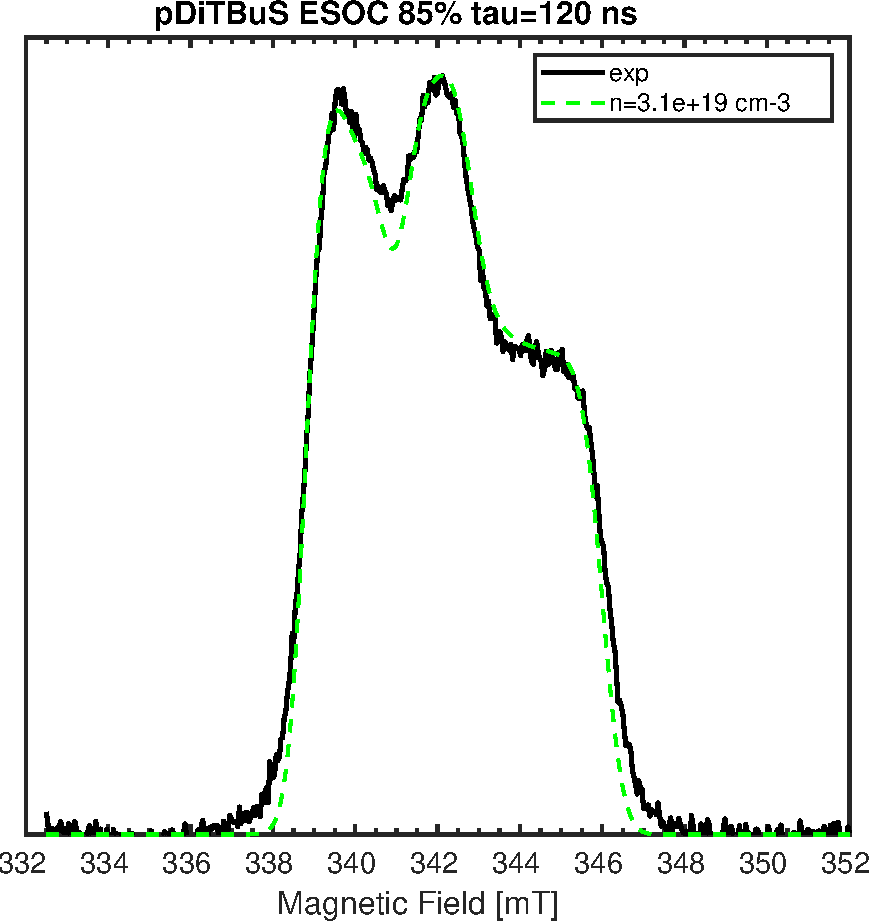
\includegraphics[width=0.5\textwidth]{./pulse/figures/Figure_S23.pdf}
	\caption{EDFS spectrum of pDiTBuS at 85\%~ESOC (solid-black). Spectral simulation with \textit{\textbf{g}}=[2.00987, 2.0055, 2.0026],\textit{\textbf{A}}=[22.0 21.5 96.3], 0.81~mT (lwpp) \ik{Gaussian} line shape and anisotropic relaxation caused by instantaneous diffusion (dashed-green). Relative peak intensities correspond to C=3.1e19 cm$^{-3}$ or 52~\si{\milli\Molar}. Microwave frequency: 9.6~GHz, $\pi/2=20$~ns, $\tau$=120~ns. Temperature: 5~K.}
	\label{fig:Figure_S23}
\end{figure}


\newpage


\subsection{Instantaneous Diffusion in PDiTBuS at ESOC~95\% }
\label{esi:fse_sims_ID_full}
The asymmetric EDFS spectrum of pDiTBuS at 95\% ESOC could not be simulated considering the distortion of the standard TEMPO spectrum caused by the ID given by Eq. \ref{eq:inst_diff} in the main text. The spectrum and the attempted fit are shown in Figure~\ref{fig:Figure_S_SIM_FSE_SOC95_ID}. The low-field peak has a much higher relative intensitiy than expected from the ID model. The observed spectrum may be a superposition of a dilute species that do not experience instantaneous diffusion and the densely packed species that is affected by ID.\\

\begin{figure}[ht!]
  \centering
	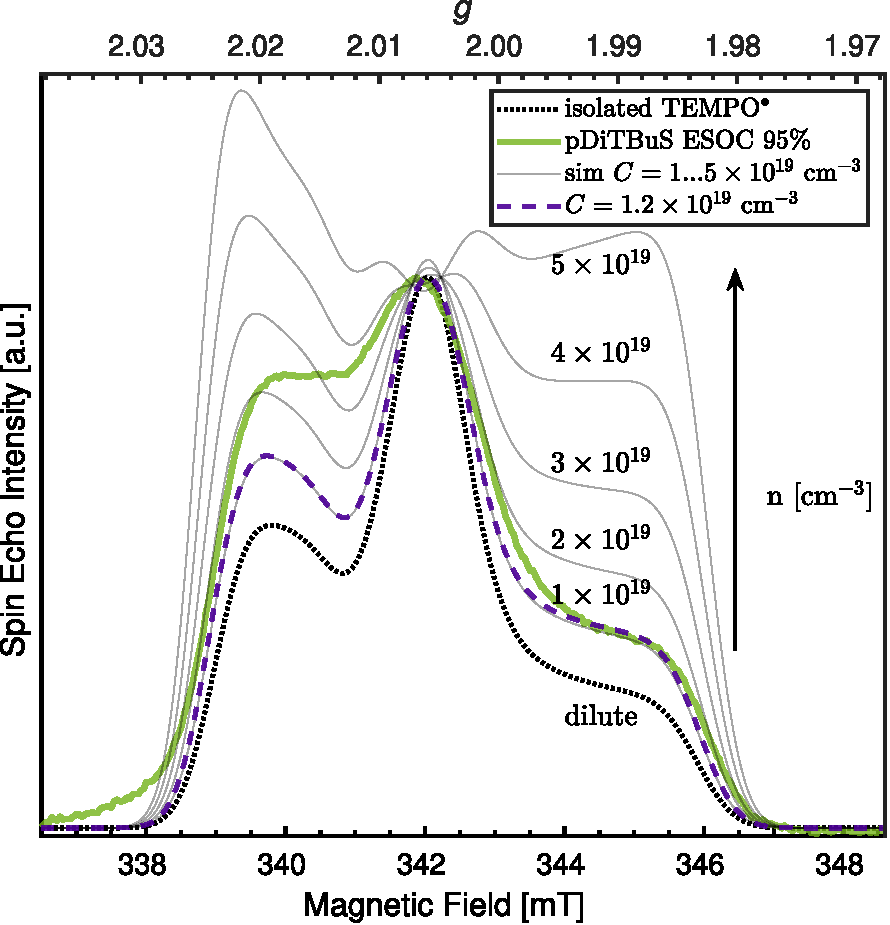
\includegraphics[width=0.5\textwidth]{./pulse/figures/Figure_S24.pdf}
	\caption{EDFS spectrum of pDiTBuS at ESOC~95\% (solid-green). Spectral simulation with \textit{\textbf{g}}=[2.0099, 2.0055, 2.0026], \textit{\textbf{A}}=[21.9850 21.4260 96.2707]~MHz, 0.24~mT (lwpp) \ik{Lorentzian} line shape and anisotropic relaxation caused by instantaneous diffusion (dashed-blue). Relative peak intensities correspond to C$=1.2\times10^{19}$~cm$^{-3}$ or 22~\si{\milli\Molar}. Microwave frequency: 9.6~GHz, $\pi/2=20$~ns, $\tau$=120~ns. Temperature: 5~K.}
	\label{fig:Figure_S_SIM_FSE_SOC95_ID}
\end{figure}

\newpage




\subsection{Estimation of Local Spin Concentrations}



\section{Spin Relaxation in charged pDiTBuS}
\label{S:RELAX_TIMES}

As we have shown in Section~\ref{S:ID}, the reason for the distorted spectral shape in pDiTBuS at ESOC~85\% is instantaneous diffusion that manifests itself in anisotropic spin relaxation which alters the \rs{relative} peak intensities. However, the spectrum \rs{for} ESOC~95\% cannot be simulated assuming just instantaneous diffusion (cf. Figure~\ref{fig:Figure_S_SIM_FSE_SOC95_ID}, ESI). In order to gain additional information about the processes that may influence the shape of the EDFS spectra, we \ik{performed field-dependent measurements of \rs{the} spin relaxation times.}\\

Figure~\ref{fig:Figure_5}a shows the EDFS spectra of pDiTBuS for 85\% and 95\% ESOC as well as a reference sample (50 mM solution of TEMPOL in Dichloromethane:Acetonitrile (3:1) glass) measured at $T=5$~K. The spectra reveal markedly different intensities of the three hyperfine components.\\

\begin{figure*}[ht]
	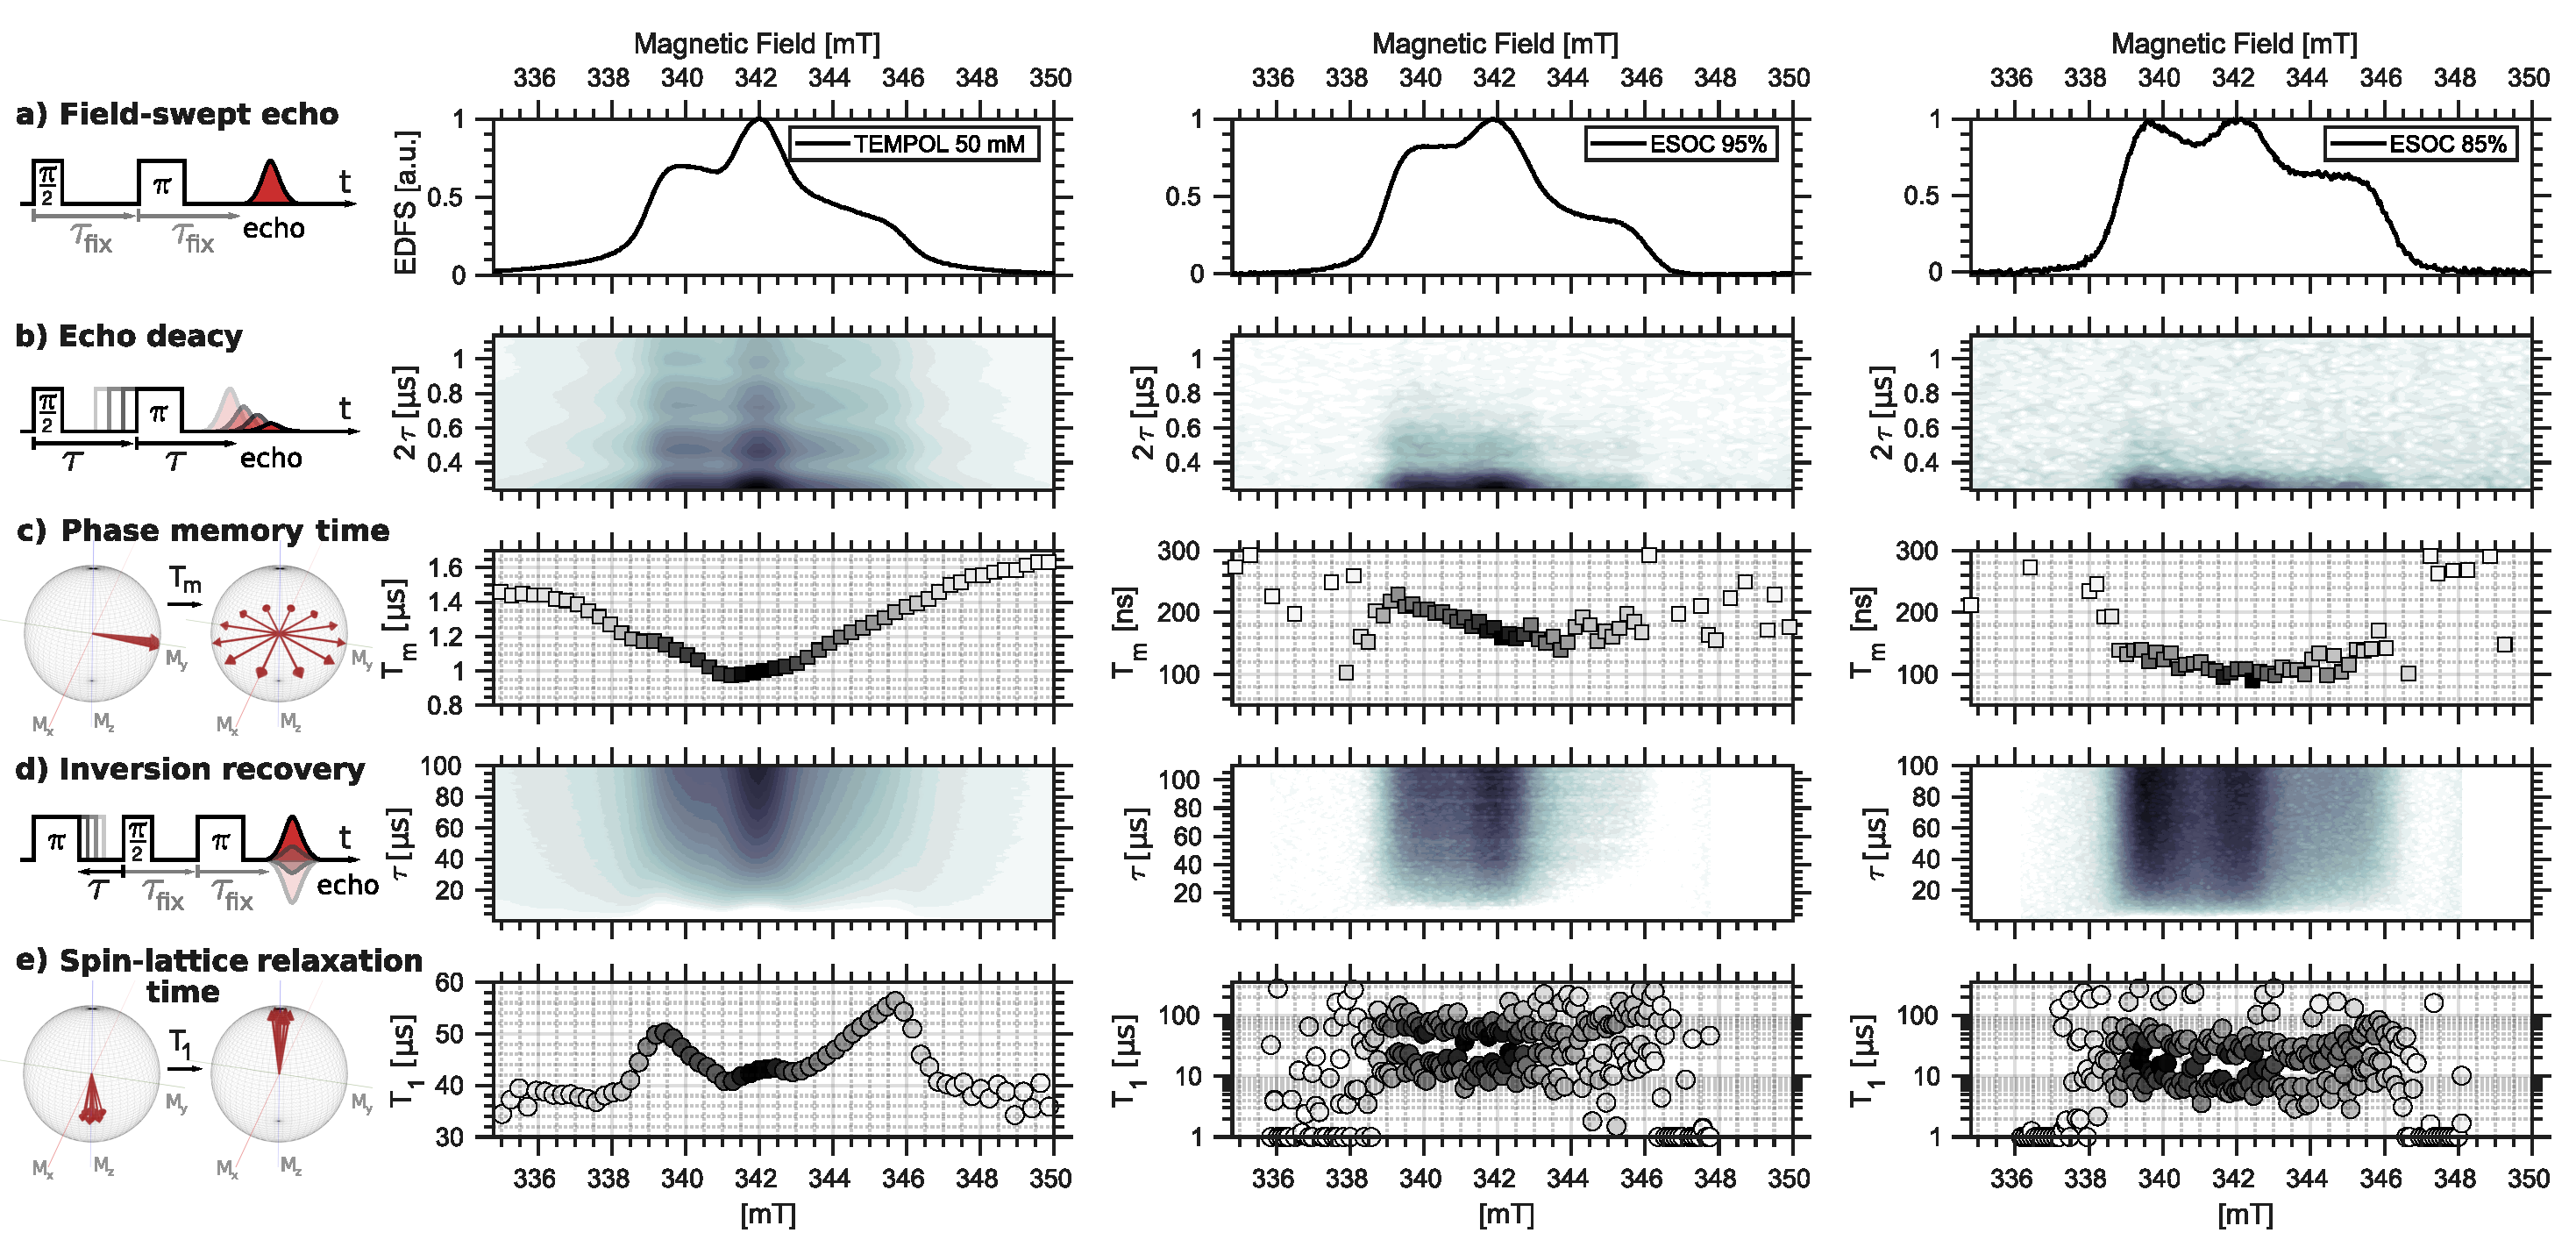
\includegraphics[width=1\textwidth]{./pulse/figures/Figure_5.pdf}%FSE_DTBS_Figure_5nl.pdf}
	\caption{Field-swept echo (a), echo decay transients (b), phase memory times $T_m$ (c), inversion recovery (d) and spin-lattice relaxation times $T_1$ (e) measured in 50~\si{\milli\Molar}  frozen electrolyte solution of TEMPOL~(left) and in dry pDiTBuS film charged to ESOC~95\%~(center) and to ESOC~85\%~(right). Temperature 5~K. \q{Grayscale} represents the intensity in b)$-$e).}
	\label{fig:Figure_5}
\end{figure*}


\rs{The changed relative peak intensities in pDiTBuS may be the result of a magnetic field-dependent spin relaxation mechanism that manifests itself in a field-dependent phase memory time $T_m$~\cite{Schweiger2001}. The $T_m$ for pDiTBuS and for TEMPOL was probed in a field-swept echo decay experiment}. The echo decay transients for the three samples are shown in Figure~\ref{fig:Figure_5}b. A \q{Hahn echo} pulse sequence was used with a $\pi/2$ pulse length of 20~ns and variable pulse separation time $\tau\geq120$~ns. Spin echo was detected at 2$\tau$ after the $\pi/2$ pulse. Periodic oscillations in the echo decay transients correspond to the ESEEM effect from protons~\cite{Schweiger2001} with $\Delta\omega_L\approx15$~MHz, which are particularly pronounced for TEMPOL.\\ 

If the sample contains several different species (i.e. nitroxide radicals in different environments and/or different local concentration) with distinct spin-spin relaxation times, the echo decay transients may contain multiple decay components, so more than one $T_m$ can correspond to each field point. This effect is not considered when simulating the effect of instantaneous diffusion using Equation~\ref{eq:inst_diff}. To determine the number of decay components in the echo decay transients, we studied the poles of the Pad{\'e} approximation of the Taylor expansion of the Laplace transforms \ik{of the transients that is} known as the Pad{\'e}-Laplace method~\cite{Hellen2005} (see ESI, Section~\ref{pade_laplace_T2} for details). This analysis revealed only monoexponential spin echo decays for both 95\%~ESOC and 85\%~ESOC. We therefore assumed a monoexponential spin echo decay for pDiTBuS\ik{, though some faster relaxing components with \rs{$T_m<t_d$} might have decayed by the earliest achievable $\tau$}\rs{, as shown in Section~\ref{esi:dead_time}, ESI.} The detected decay times $T_m(B_0)$, extracted from fits of the background-corrected echo-decay curves, are shown in Figure~\ref{fig:Figure_5}c as filled squares with \q{the grayscale} representing the amplitude of the corresponding fit component. \q{As expected, $T_m$ is significantly larger for 95\% than for 85\% ESOC, consistent with the weaker spin-spin couplings in the fully charged film. Further, we note that the field-dependence of $T_m$ is more pronounced for 95\% ESOC, with $T_m\geq200$~ns for the $m_I=+1$ hyperfine component. This anisotropy in $T_m$ results in an increased intensity of the low-field peak, which is in line with the observation that we cannot describe the 95\% ESOC spectrum assuming only instantaneous diffusion (see Section~\ref{S:ID}).} The transient fits and the residuals are shown in Section~\ref{pade_laplace_T2}, ESI.\\

We attempted to reproduce the pDiTBuS spectra from a standard nitroxide spectrum by considering anisotropic transient decay of the spectral intensity at \ik{$t=\tau=120$~ns for each $B_0$} with the measured $T_m(B_0)$. However, this approach did not allow us to reconstruct the pDiTBuS spectra for neither 85\%, nor 95\%~ESOC.\\

% The measured $T_m$ is more anisotropic for the 95\%~SOC.\\ 


It was recently shown, that densely packed TEMPO radicals in a TEMPO-containing, non-conductive polymer PTMA, intermixed into \q{an} amorphous carbon mesh, show multi\ik{ple} spin-lattice relaxation times $T_1$ because of different types of contact between the TEMPO radicals and the conductive additive in the TEMPO/carbon composite~\cite{Daniel2023}. In order to find out whether such behavior can also be observed for \ik{the porous} pDiTBuS film, we measured spin-lattice relaxation times $T_1$ with an inversion-recovery pulse sequence ($\pi-\tau-\pi/2-\tau_{fix}-\pi-\tau_{fix}-echo$) with variable $\tau$ (Figure~\ref{fig:Figure_5}d). The Pad{\'e}-Laplace analysis yielded one decay component for TEMPOL and two decay components for pDiTBuS both at 85\%~ESOC and 95\%~ESOC (see ESI, Section~\ref{esi:pade_laplace_T1} for details). The $T_1$ for charged pDiTBuS is \w{on the same order as for }TEMPOL and splits in two rather broad distributions with \w{similar} intensities (Figure~\ref{fig:Figure_5}e). \q{Similar as in the case of $T_m$, also $T_1$ is larger for 95\% than for 85\% ESOC. Irrespective of the ESOC there is no significant field dependence of $T_1$, in contrast to what is observed for the TEMPOL reference sample.\\} 

Daniel et al.\q{~\cite{Daniel2023}} concluded that separate distributions of $T_1$ correspond to different \ik{binding between TEMPO and the carbon mesh, representing the} quality of electrical contact between TEMPO and the conductive additive. With the observed distribution of $T_1$ and considering the two-component cwEPR spectral contributions for charged pDiTBuS \ik{(``broad'' and ``dilute'' components, cf. Section~\ref{esi:cw_sims}, ESI)}, we suggest \rs{that two types of domains could exist} in a \ik{partially} charged pDiTBuS film \rs{as well. These two} \ik{morphologies \rs{may correspond to} \q{``conductive''} domains with shorter $T_1$, where TEMPO$^{\bullet}$ are close to the conductive pNiSalen backbone, and \q{``non-conductive''} domains with longer $T_1$, where TEMPO$^{\bullet}$ are separated from pNiSalen}. \rs{We note, however, that based on the experimental data presented here, this interpretation is rather speculative.} \ik{The detected $T_1$ values for pDiTBuS may also correspond to one distribution, as the separation between the $T_1$ values is comparable to \rs{the widths of their distributions}}.\\%NiSalen backbone.\\

\subsection{Temperature Dependence of pEPR Spectra of pDiTBuS}
Spin relaxation times usually depend on temperature\ik{\cite{Schweiger2001}}. We measured EDFS of charged pDiTBuS at \rs{5~K} and at \rs{80~K} to see how faster spin relaxation affects the spectral shape. Figure~\ref{fig:Figure_6} shows EDFS spectra for pDiTBuS \ik{ charged to} ESOC~95\% (a) and \ik{to} ESOC~85\% (b) \ik{at 80~K (solid) and at 5~K (dashed)}. At 80~K an overnight scan was required to obtain a satisfactory signal-to-noise ratio, \rs{whereas} at 5~K the spectrum was recorded in a few minutes. The spectral intensities at different temperatures were \ik{scaled} \rs{such that} the high-field $m_I=-1$ peak \rs{has the same intensity}. Figure~\ref{fig:Figure_6} clearly shows that the relative intensities of the peaks change with temperature for both ESOC. At higher temperatures the EDFS spectrum of pDiTBuS has a peak ratio closer to that of dilute TEMPOL that corresponds to \ik{a} lower spin concentration\ik{,} according to Equation~\ref{eq:inst_diff}. The influence of the temperature \ik{increase} on the spectral shape is stronger for the \ik{lower,} 85\% ESOC.

\begin{figure}[ht]
\center
	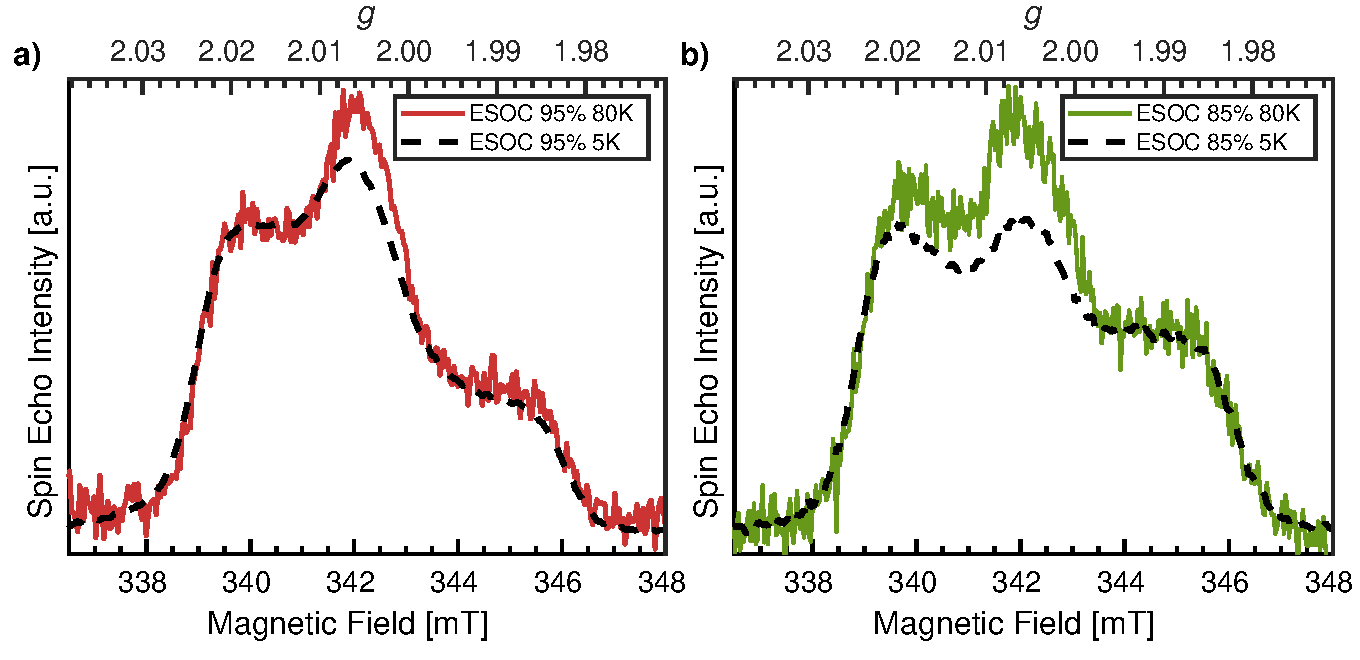
\includegraphics[width=0.9\textwidth]{./pulse/figures/Figure_6.pdf}
	\caption{EDFS spectra for pDiTBuS charged to 95\%\ik{~ESOC} (a) and to 85\%\ik{~ESOC} (b) measured at 5K and at 80K.}
	\label{fig:Figure_6}
\end{figure}


The overall relaxation times in the film decrease with \ik{increasing} temperature, but the dead time of the spectrometer ($t_d=120$~ns) does not change. Therefore, at a given temperature, only \ik{spins with $T_m>t_d$} contribute to the signal. At higher temperature only the weakly coupled spins \ik{(with the longest $T_m$)} are detectable, which results in a spectral shape that is \q{less affected by instantaneous diffusion and thus }closer to a dilute nitroxide solution.\\

\subsection{\ik{Limitation on Shortest Detectable $T_m$ by the Spectrometer Dead Time}}
\label{esi:dead_time}

\ik{If a system exhibits multiple phase memory times $T_m$, the spin echo from the species with short memory times may decay below the noise level at a given pulse separation $\tau$. Figure~\ref{fig:Figure_S25} illustrates the spin echo intensity in a two-component system with $T_m^1=100$~ns and $T_m^2=25$~ns in dependence on the pulse separation $\tau$. The fast relaxing component with $T_m^2=25$~ns decays below the noise level after the dead time of $t_d=100$~ns.}

\begin{figure}[h]
\center
	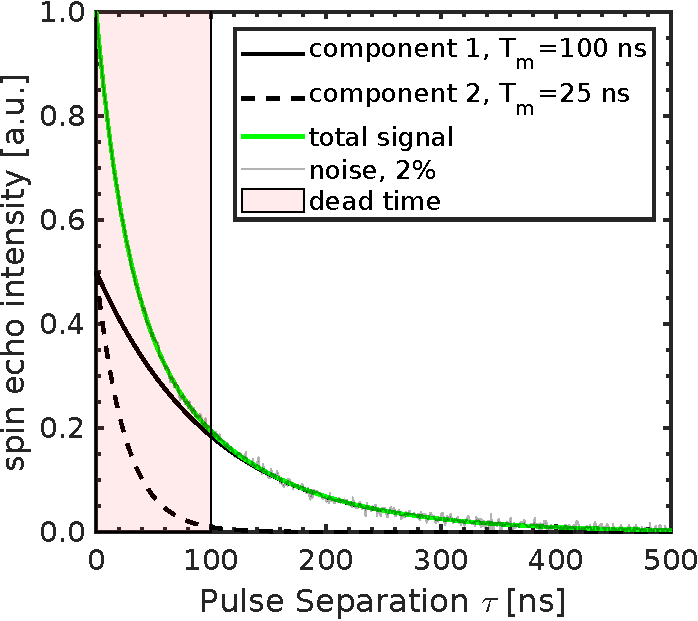
\includegraphics[width=0.4\textwidth]{./pulse/figures/Figure_S25}
	\caption{\ik{Simulated echo decay transient of a spin ensemble exhibiting two distinct phase memory times $T_m^1=100$~ns and $T_m^2=25$~ns. The 100~ns dead time, during which the spin echo detection is not possible, is marked in red. After the dead time, the sum of the two components is indistinguishable from the slowly relaxing component within the 2\% noise.}}
	\label{fig:Figure_S25}
\end{figure}


\section{Pad{\'e}-Laplace Deconvolution of Polyexponential Decay Signals}
\label{sec:pade-laplace}
The echo decay and inversion recovery transients measured in the corresponding experiments may contain multiple exponential decay components. The conventional method of determining the distribution of the decay components in a transient decay is the Laplace inversion, where the signal in the time domain $s(t)$ is converted into its Laplace image $L(p)=\int\limits_{0}^{+\infty}s(t)e^{-pt}\mathrm{d}t$ in the time-constant domain $p=1/t$, where the peaks of $L(p)$ give the decay constants that make up the signal. However, for the noisy signal, the direct calculation of the Laplace transform brings in artifacts that drastically vary with the noise. The signal-to-noise ratio (SNR) of the recorded data makes it difficult to apply the Laplace inversion to determine the number of the decay components, as the Laplace transform is unstable at that SNR. \\ 


The Pad{\'e}-Laplace method comes useful for analyzing noisy polyexponential decays as it was demonstrated in Ref.~\cite{Hellen_2005}. The idea of the Pad{\'e}-Laplace method is to analyze the Pad{\'e} approximation of the Taylor expansion of the $L(p)$ in the vicinity of one of the expected decay constants $p_0$, rather than considering the $L(p)$ fully. This way of signal decomposition is stable against the noise for SNR$<$10 (see Figure~\ref{fig:Figure_S7}). The number of exponents detected by the Pad{\'e}-Laplace method as well as their locations in the $p$ space may vary depending on the expansion point $p_0$. We considered $p_0=1/t_{1/2}$ where $t_{1/2}$ is the time at which the signal amplitude halves.\\

We implemented the following algorithm to detect the number of exponents in the decaying transient $s(t)$:\\

First, a point $p_0=1/t_{1/2}$ was chosen, at which $s(t)$ halves.\\

Then, 11 coefficients of the Taylor expansion of the Laplace transform $L(p)$ were calculated in the vicinity of $p \rightarrow p_0$\\

\begin{equation}
L(p)\vert_{p \rightarrow p_0} = \sum_{n=0}^{11} d_i (p-p_0)^i
\end{equation}
with
\begin{equation}
d_i = \frac{1}{i!}\left(\frac{d^{(i)}L}{dp^{(i)}}\right)_{p=p0}
\end{equation}
where the derivatives $\frac{d^{(i)}L}{dp^{(i)}}$ are computed numerically at the point $p=p_{0}$ from the discrete signal $s(t) = (t_j,f_j),~j=1~...~M$:
\begin{equation}
\frac{d^{(i)}L}{dp^{(i)}}= \sum_{j=2}^{M-1}(-t_j)^ie^{(-p_0t_j)}f_j + \frac{1}{2}\left((-t_1)^ie^{(-p_0t_1)}f_1+(-t_M)^ie^{(-p_0t_M)}f_M \right)
\end{equation}


Then the Taylor expansion for $L(p)$ was approximated in the vicinity of $p_0$ with the Pad{\'e} polynomials a(p) and b(p) of orders $n=5$ and $n=6$ respectively:\\

\begin{equation}
\label{eq:pade}
L(p)\vert_{p \rightarrow p_0} = d_0+d_1(p-p_0)+\dots+d_{11}(p-p_0)^{11}=\frac{a_0 + a_1(p-p_0) + \dots + a_5(p-p_0)^5}  {1 + b_1(p-p_0)+ \dots+ b_6(p-p_0)^6}
\end{equation}

The equation \ref{eq:pade} is multiplied by the the denominator and the prefactors at $(p-p_0)^{n}$ for $n=6\dots11$ are compared. This defines a system of linear equations on coefficients $b_i$:\\


\begin{equation}\label{eq:matrix}
  \begin{pmatrix}
    d_{5} & d_{4} & d_{3} & d_2 & d_1 & d_0\\
    d_6 & d_5 & d_4 & d_3 & d_2 & d_1\\
    d_7 & d_6 & d_5 & d_4 & d_3 & d_2\\
    d_8 & d_7 & d_6 & d_5 & d_4 & d_3\\
    d_9 & d_8 & d_7 & d_6 & d_5 & d_4\\
    d_{10} & d_9 & d_8 & d_7 & d_6 & d_5
  \end{pmatrix}
       \begin{pmatrix}
   b_1\\
   b_2\\
   b_3\\
   b_4\\
   b_5\\
   b_6
   \end{pmatrix}
  =
    \begin{pmatrix}
   -d_6\\
   -d_7\\
   -d_8\\
   -d_9\\
   -d_{10}\\
   -d_{11}
   \end{pmatrix}
\end{equation}

From \ref{eq:matrix}, $b_i$ are found. The coefficients $a_i$ are found from ${d}$ and ${b}$.\\

Finally, the Pad{\'e} approximation $P=\frac{a}{b}$ is constructed and its poles are analyzed. The position of the poles reveal the decay constants. The residues at the poles may give the amplitudes of the decay components, but this was not used in the present study.

\begin{figure}[ht!]
\center
	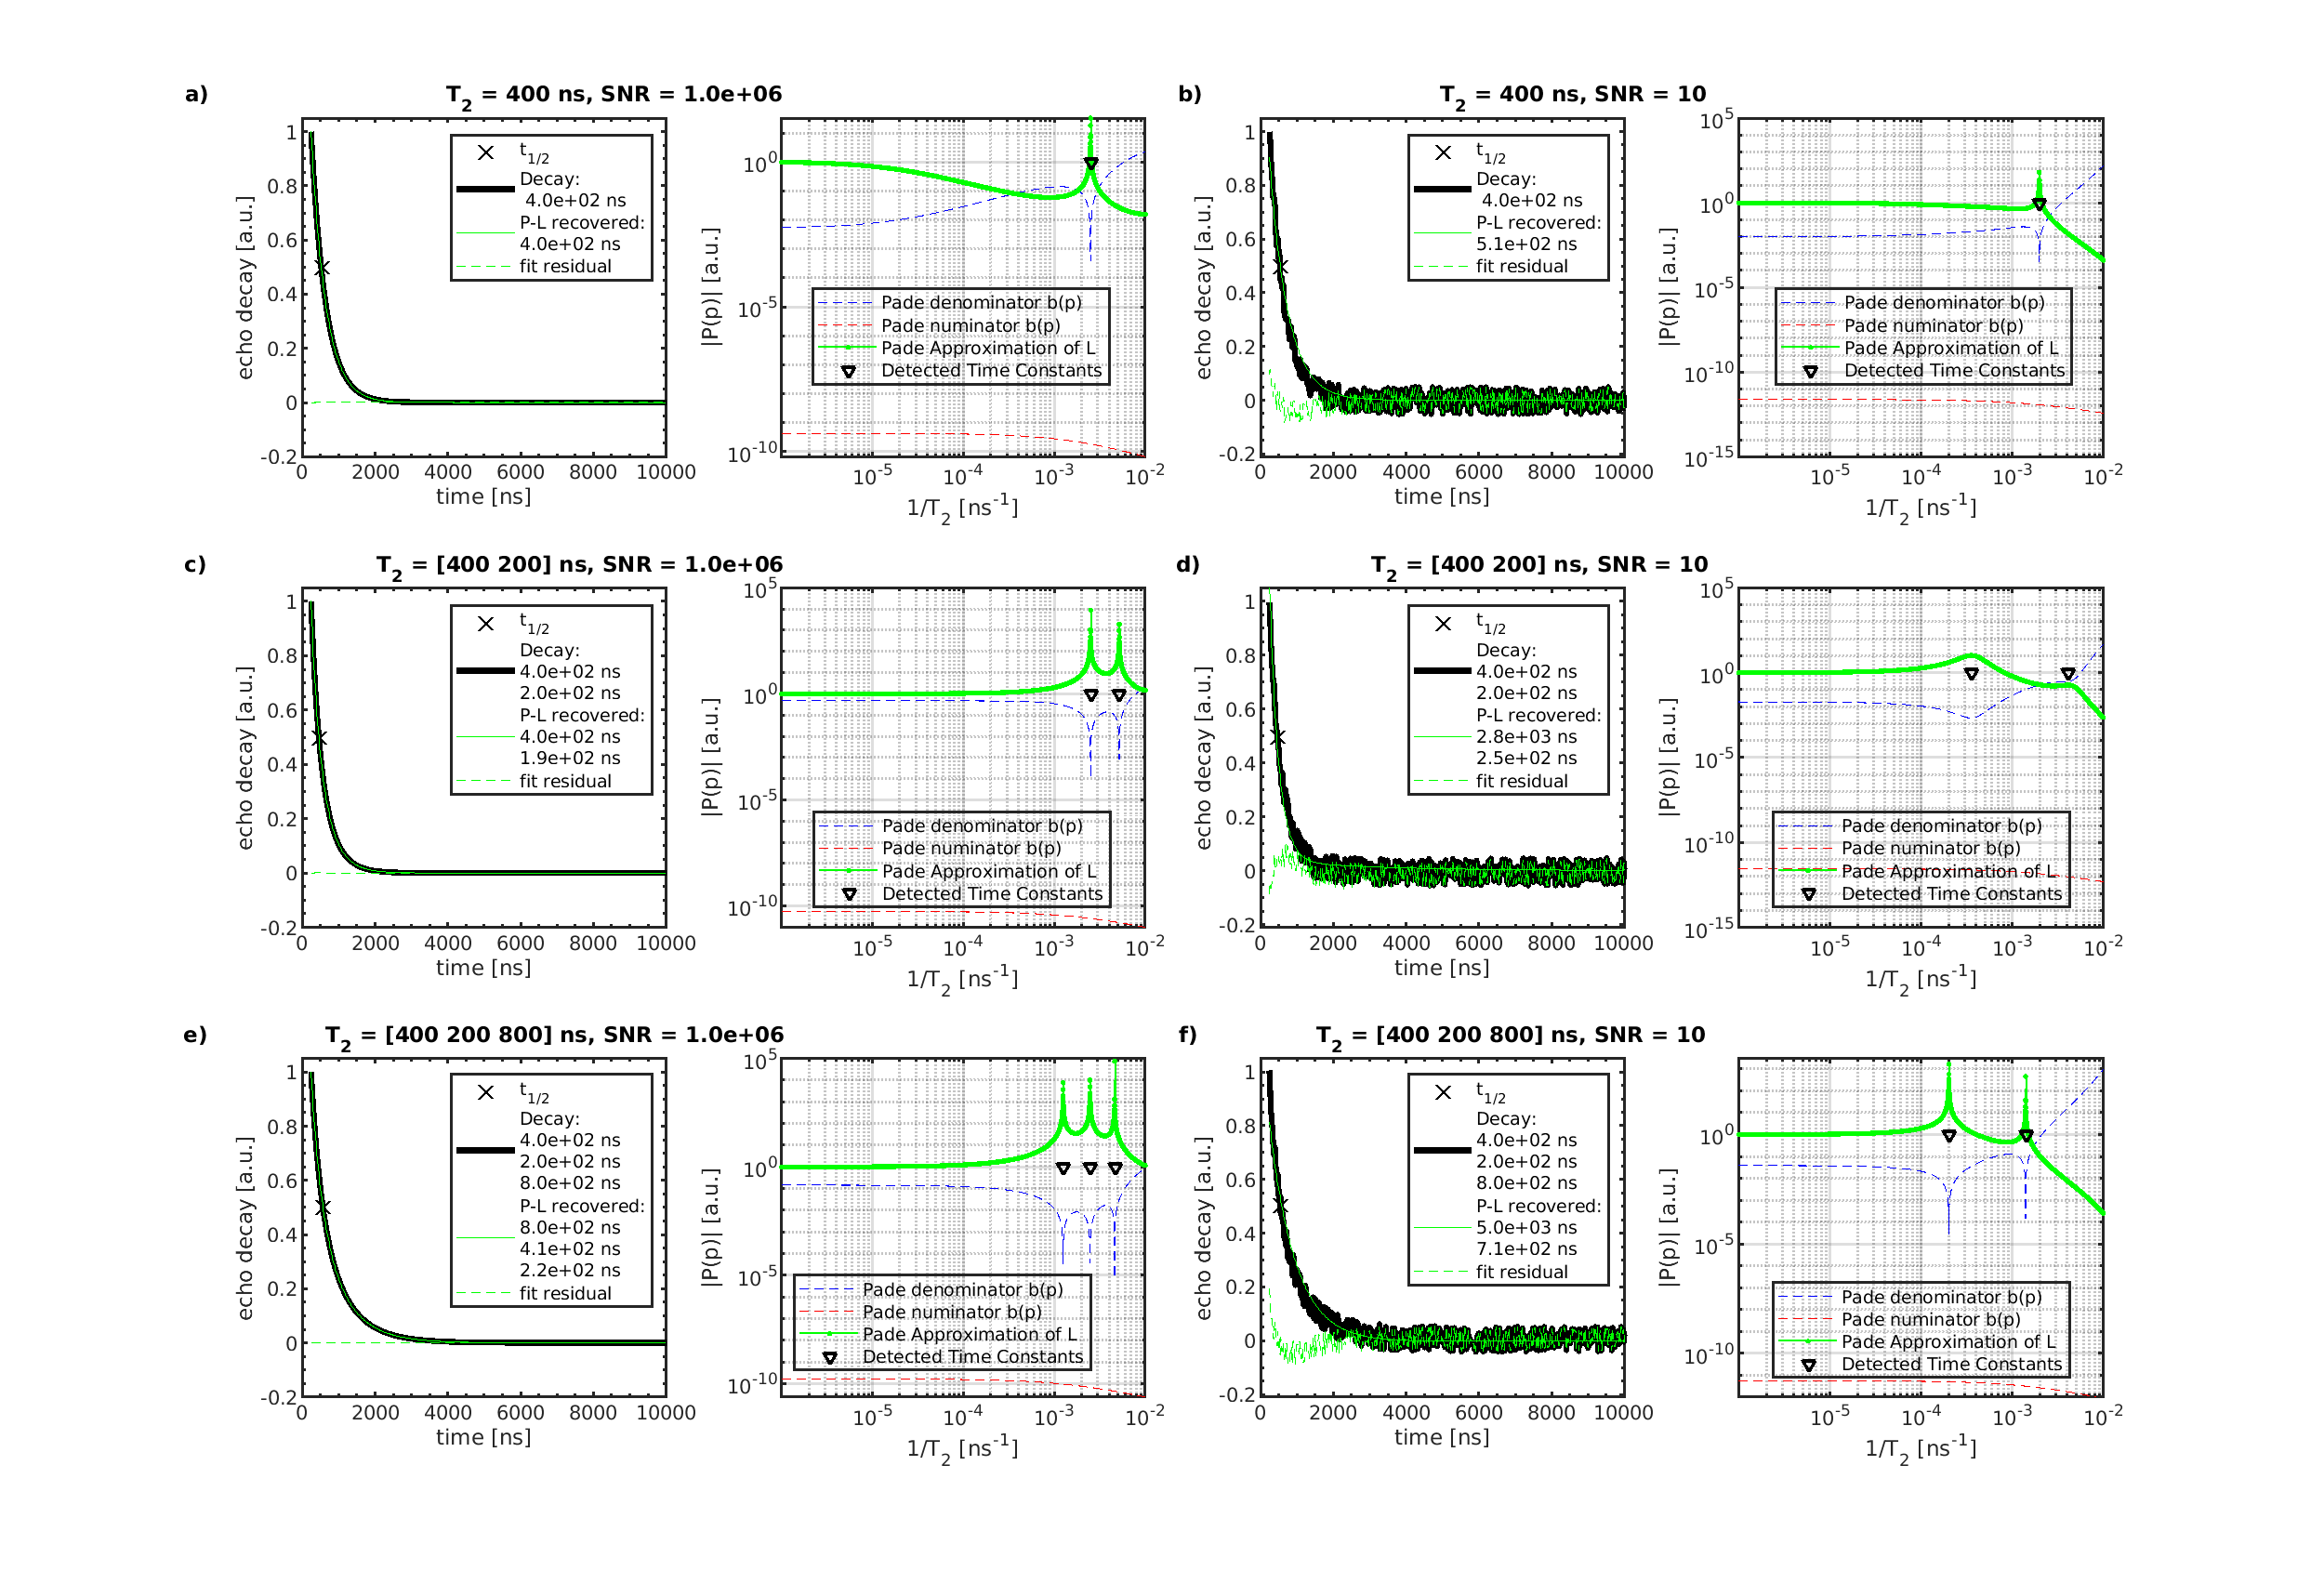
\includegraphics[width=1\textwidth]{./pulse/figures/Figure_S7.pdf}
	\caption{Pad{\'e}-Laplace deconvolution of the mock data containing two decay constants with various signal-to-noise (SNR) ratios.}
	\label{fig:Figure_S7}
\end{figure}


\newpage
\subsection{Pad{\'e}-Laplace Deconvolution of the Echo-Decay and Inversion-Recovery Transients}
\label{pade_laplace_T2}
We used the Pad{\'e}-Laplace method to determine the number of the decay constants in the signals and used multiexponential fits to adjust the decay constants and their amplitudes. For the echo decay transients the best fits were monoexponential fits, even though the Pade-Laplace analysis initially showed biexponential behavior for pDiTBuS with major contribution from the fast decay constants in the order of the detector's dead time. All recorded echo decay transients contain oscillations due to the ESEEM effect. The oscillations were excluded from the analysis as shown in the 'fit area' on the plots in Figure~\ref{fig:Figure_S9}, Figure~\ref{fig:Figure_S11} and Figure~\ref{fig:Figure_S13}.

\newpage
\subsubsection{Echo Decay in 50 mM TEMPOL}
\begin{figure}[ht!]
\center
	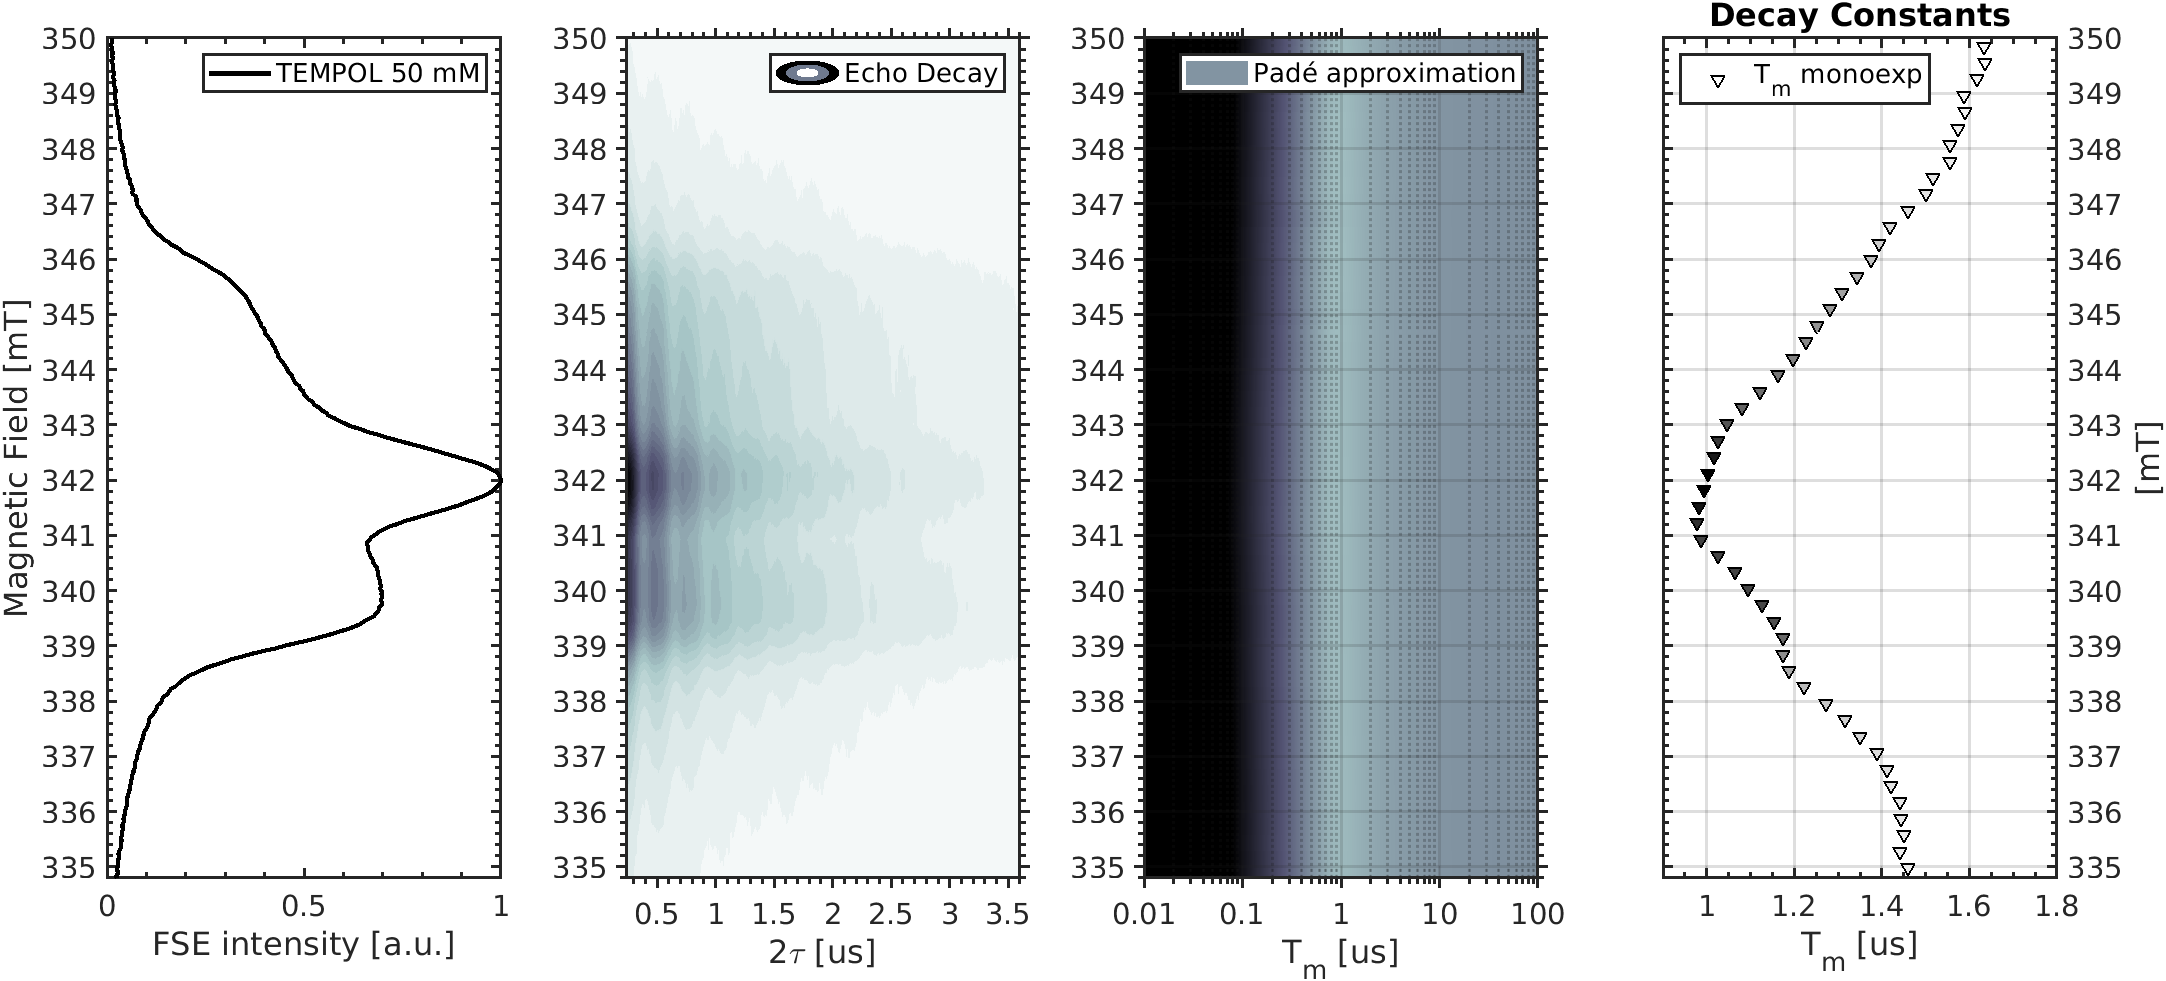
\includegraphics[width=1\textwidth]{./pulse/figures/Figure_S8.png}
	\caption{Pad{\'e}-Laplace deconvolution of the field-swept spin echo decay in a frozen 50~\si{\milli\Molar}  solution of TEMPOL in Dichloromethane:Acetonitrile glass (3:1). One decay component detected with Pade-Laplace (triangles, right panel). Monoexponential fit (squares for faster component, circles for slower component, right panel). Temperature 5K.}
	\label{fig:Figure_S8}
\end{figure}

\begin{figure}[ht!]
\center
	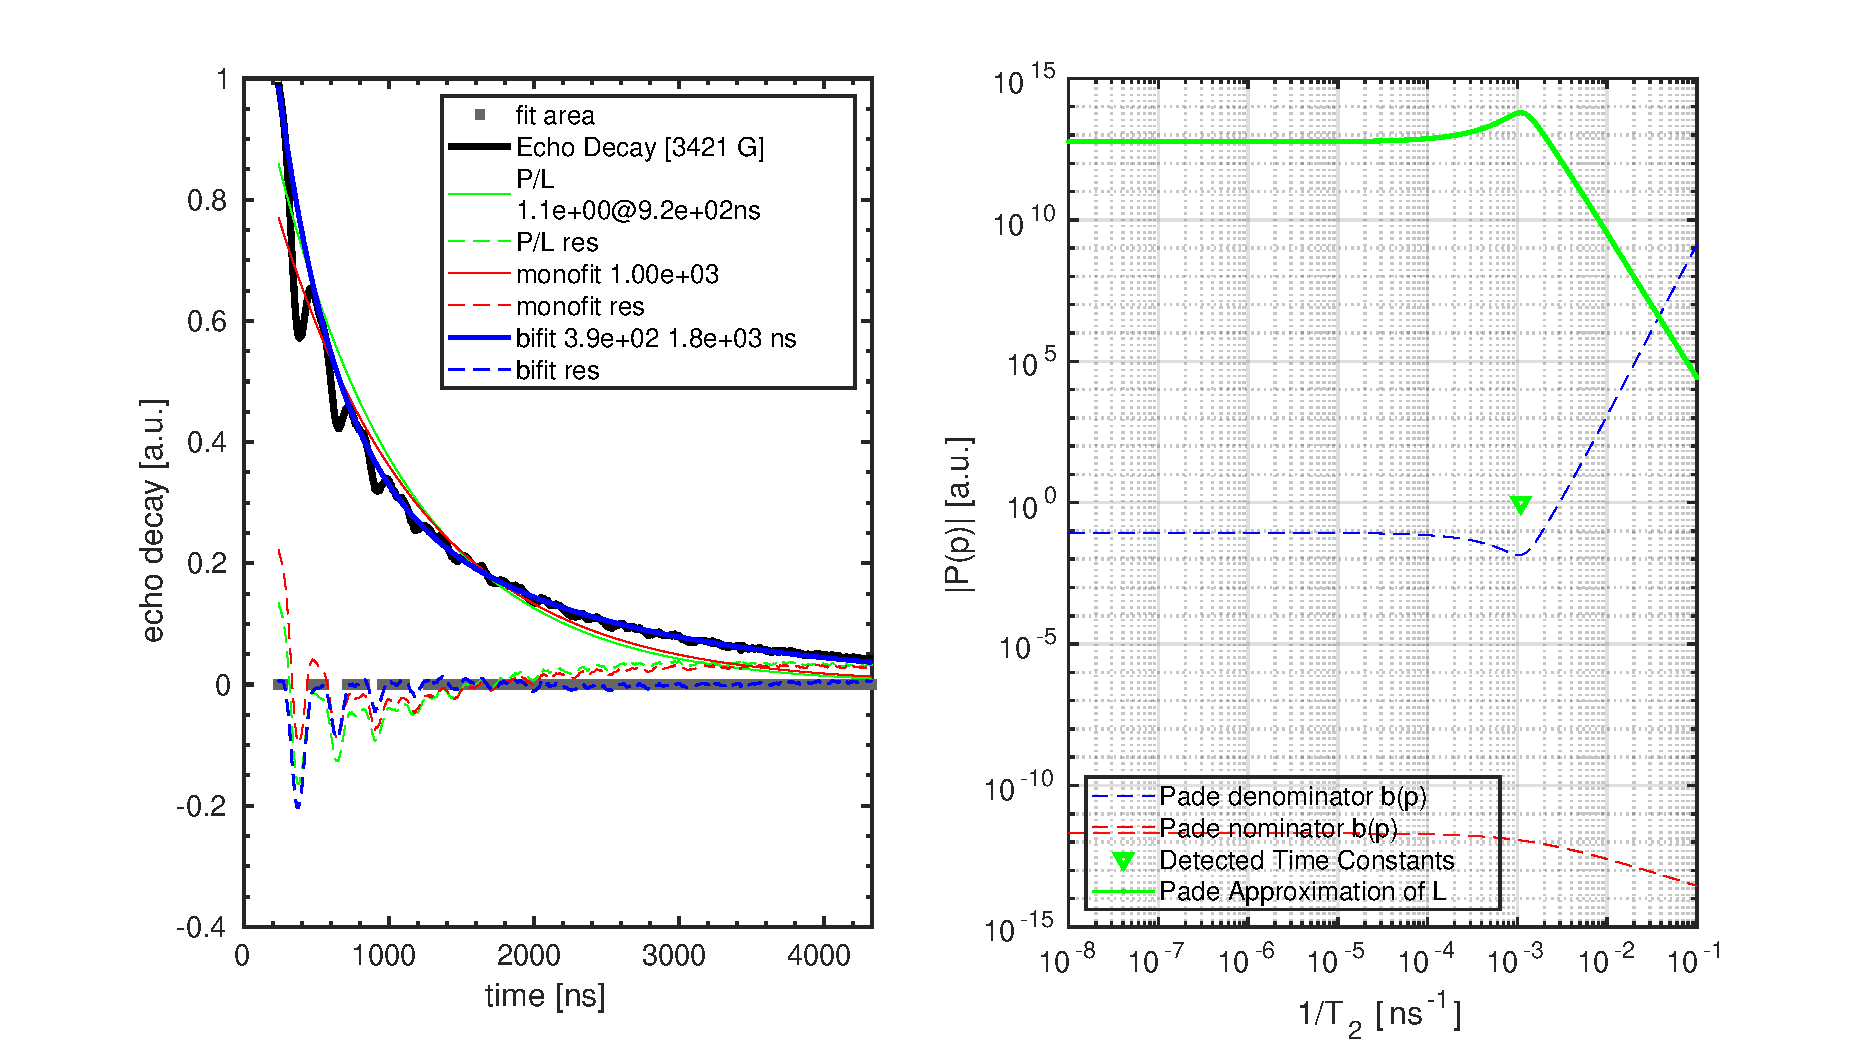
\includegraphics[width=0.5\textwidth]{./pulse/figures/Figure_S9.pdf}
	\caption{Fits of the echo decay transient in the frozen 50~\si{\milli\Molar}  TEMPOL solution at the central spectral peak ($m_I=0$, 342~mT). Pad{\'e}-Laplace deconvolution the transient vs. free monoexponential fit vs biexponential fit. Temperature 5K. Data was fit in the 'fit area' region. ESEEM oscillations were excluded from the data for fit and Pade-Laplace analysis.}
	\label{fig:Figure_S9}
\end{figure}


\newpage
\subsubsection{Echo Decay in DiTBuS 95\% ESOC}
\begin{figure}[h]
\center
	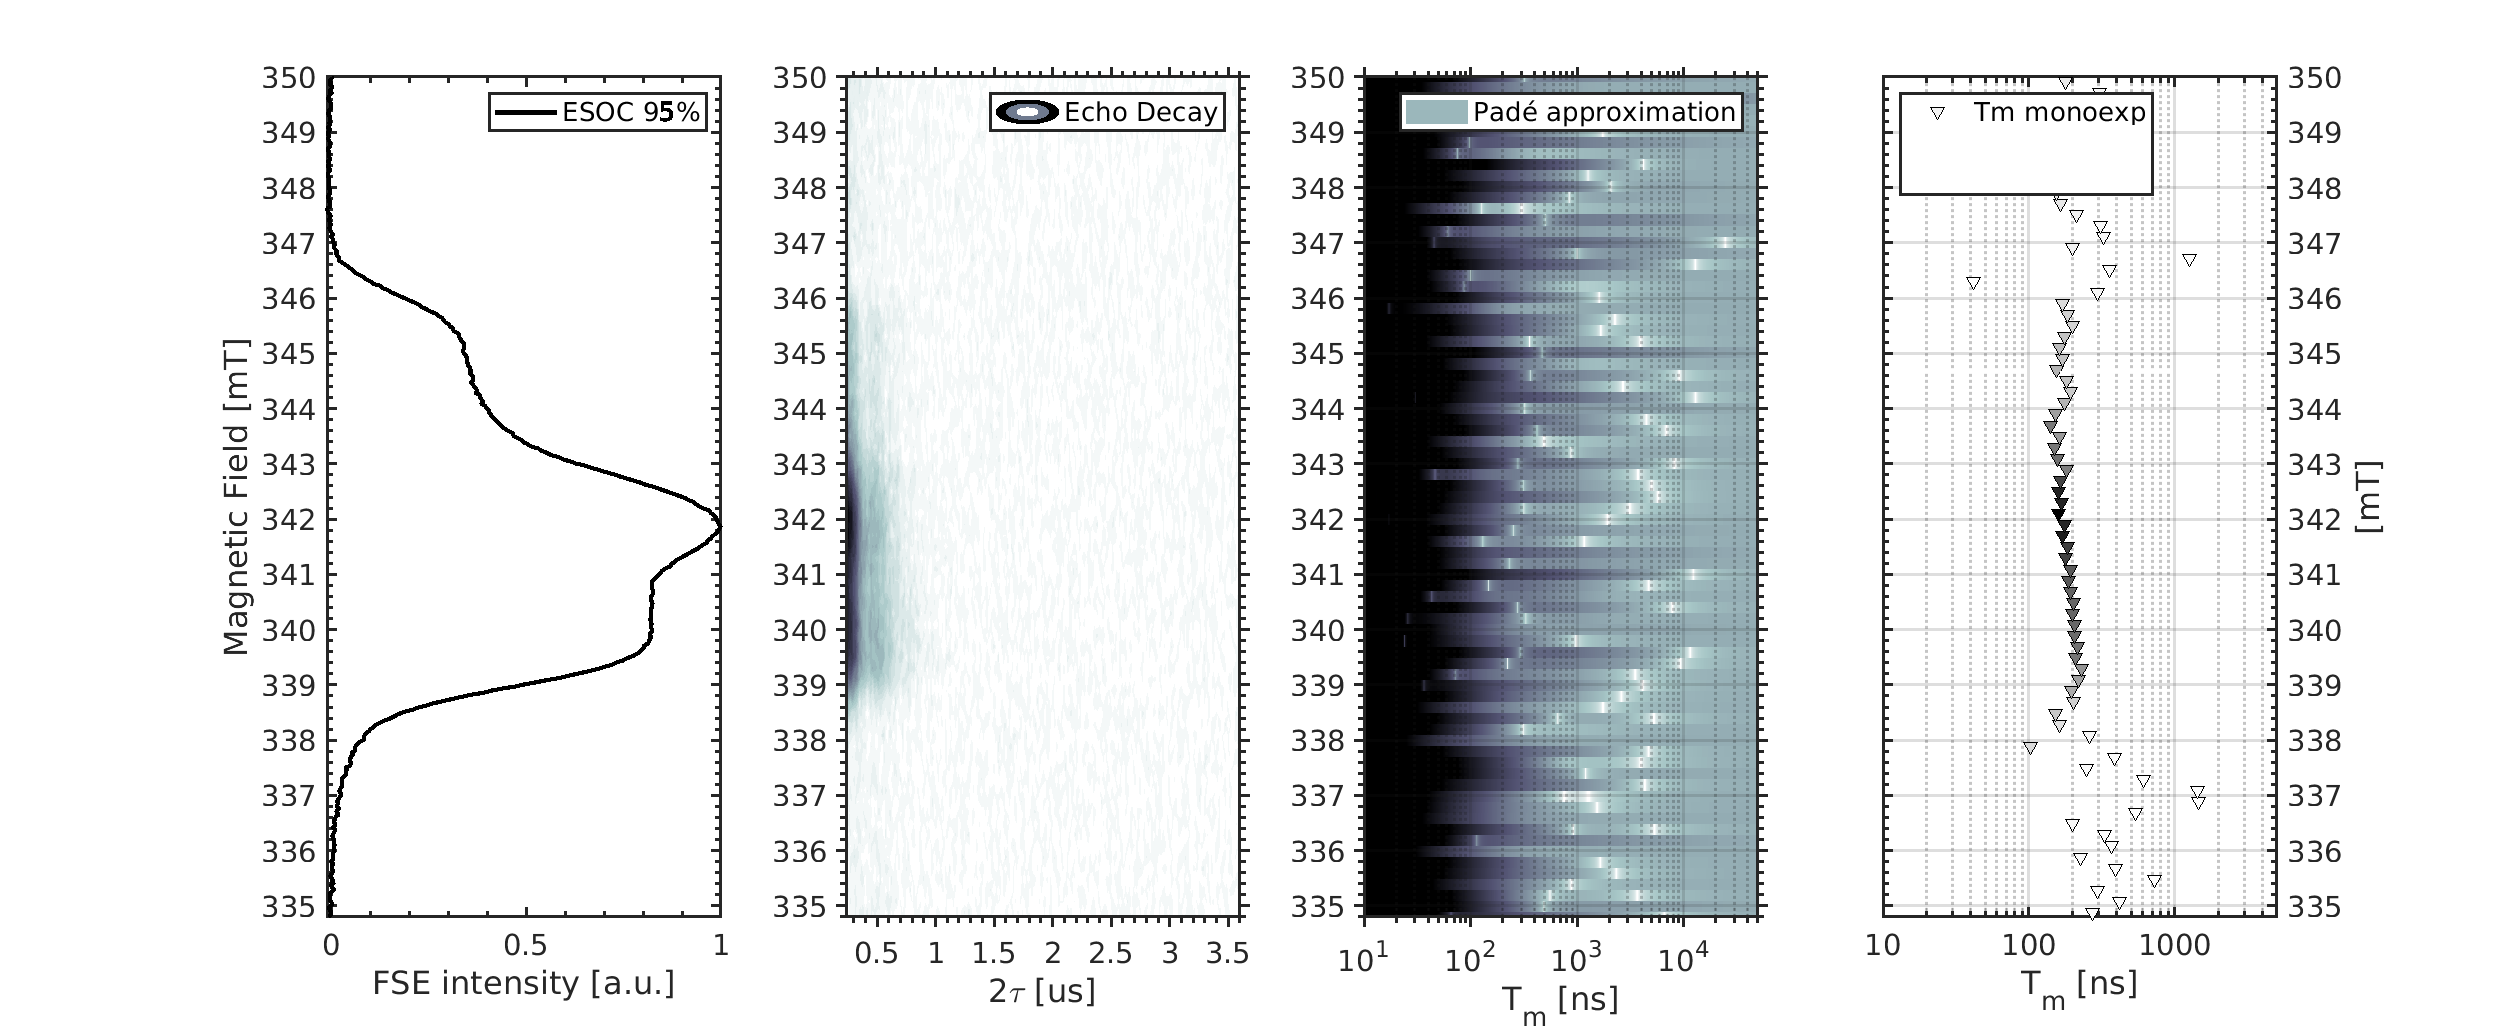
\includegraphics[width=0.5\textwidth]{./pulse/figures/Figure_S10.pdf}
	\caption{Pad{\'e}-Laplace deconvolution of the field-swept spin echo decay in the pDiTBuS film at 95\%~ESOC. Temperature 5K.}
	\label{fig:Figure_S10}
\end{figure}


\begin{figure}[ht!]
\center
	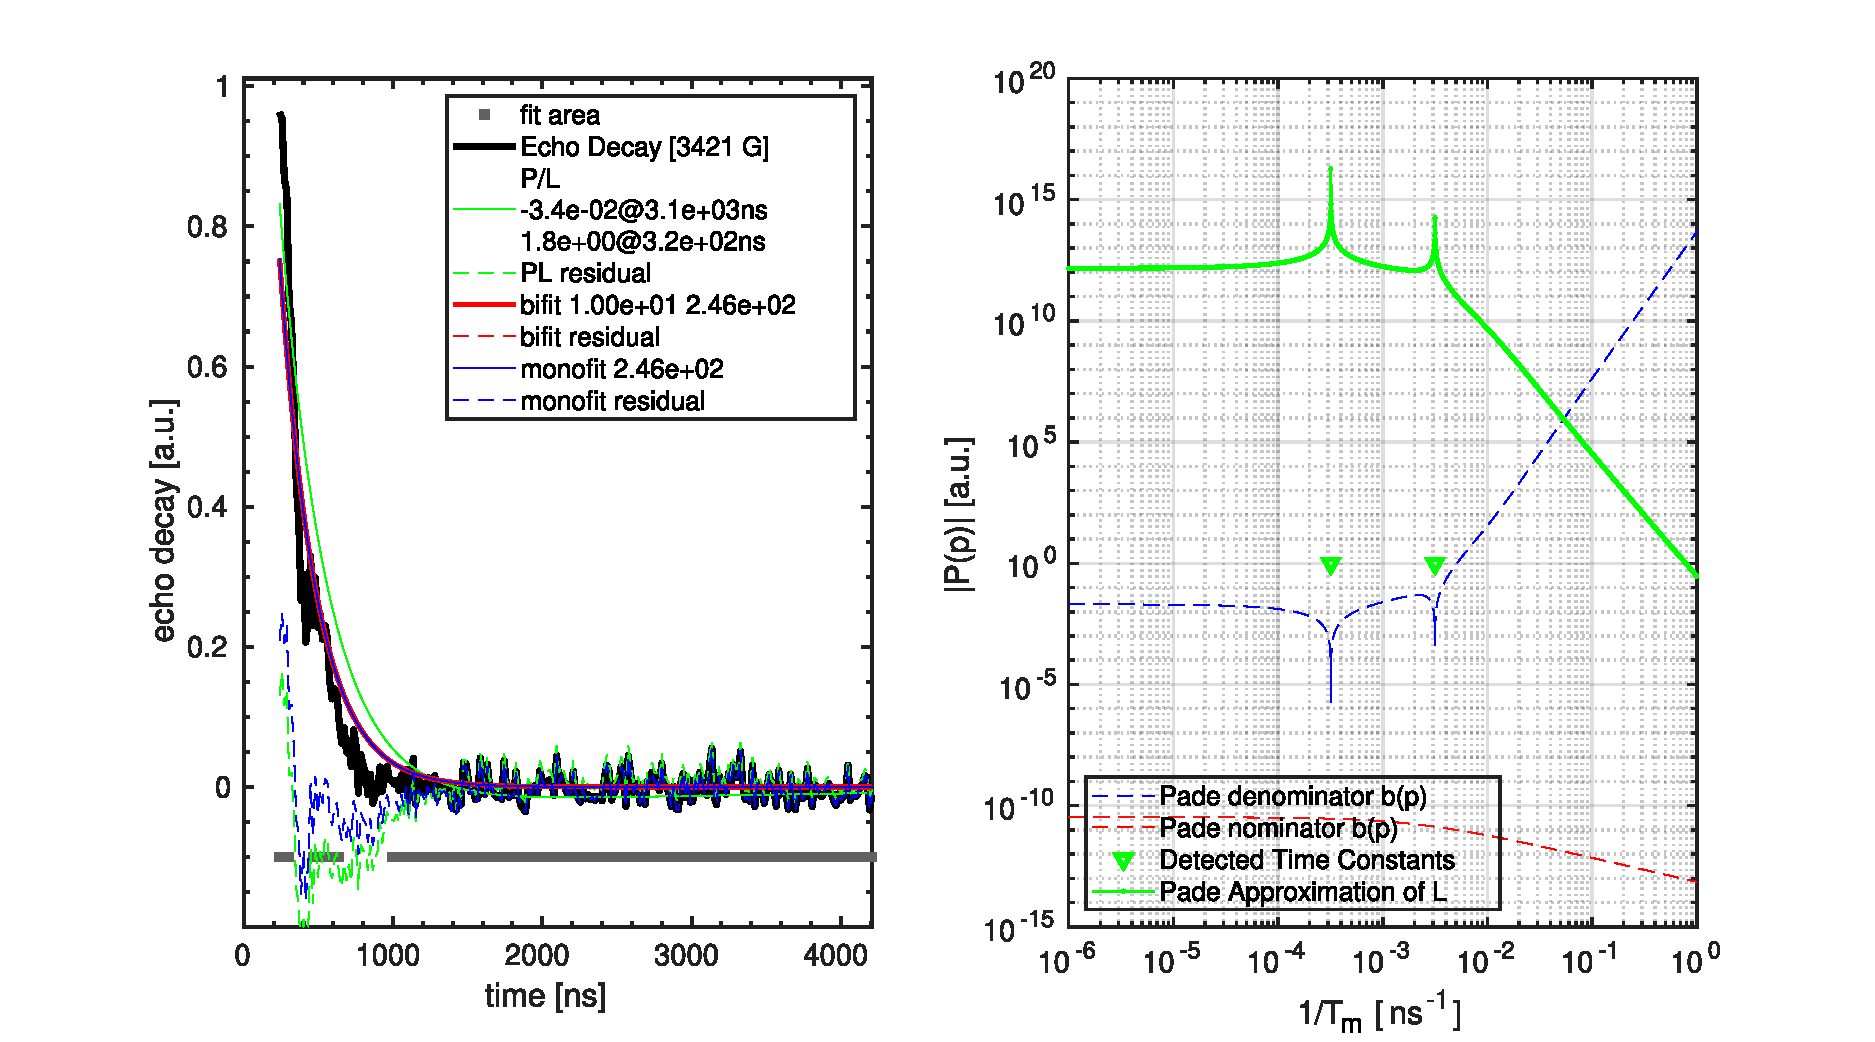
\includegraphics[width=0.5\textwidth]{./pulse/figures/Figure_S11.pdf}
	\caption{Fits of the echo decay transient in the pDiTBuS film at 95\%~SoC at the central spectral peak ($m_I=0$, 342~mT). Pad{\'e}-Laplace deconvolution the transient vs. free monoexponential fit vs biexponential fit. Temperature 5K. Data was fit in the 'fit area' region. ESEEM oscillations were excluded from the data for fit and Pade-Laplace analysis.}
	\label{fig:Figure_S11}
\end{figure}


\newpage
\subsubsection{Echo Decay in DiTBuS 85\% ESOC}

\begin{figure}[h]
\center
	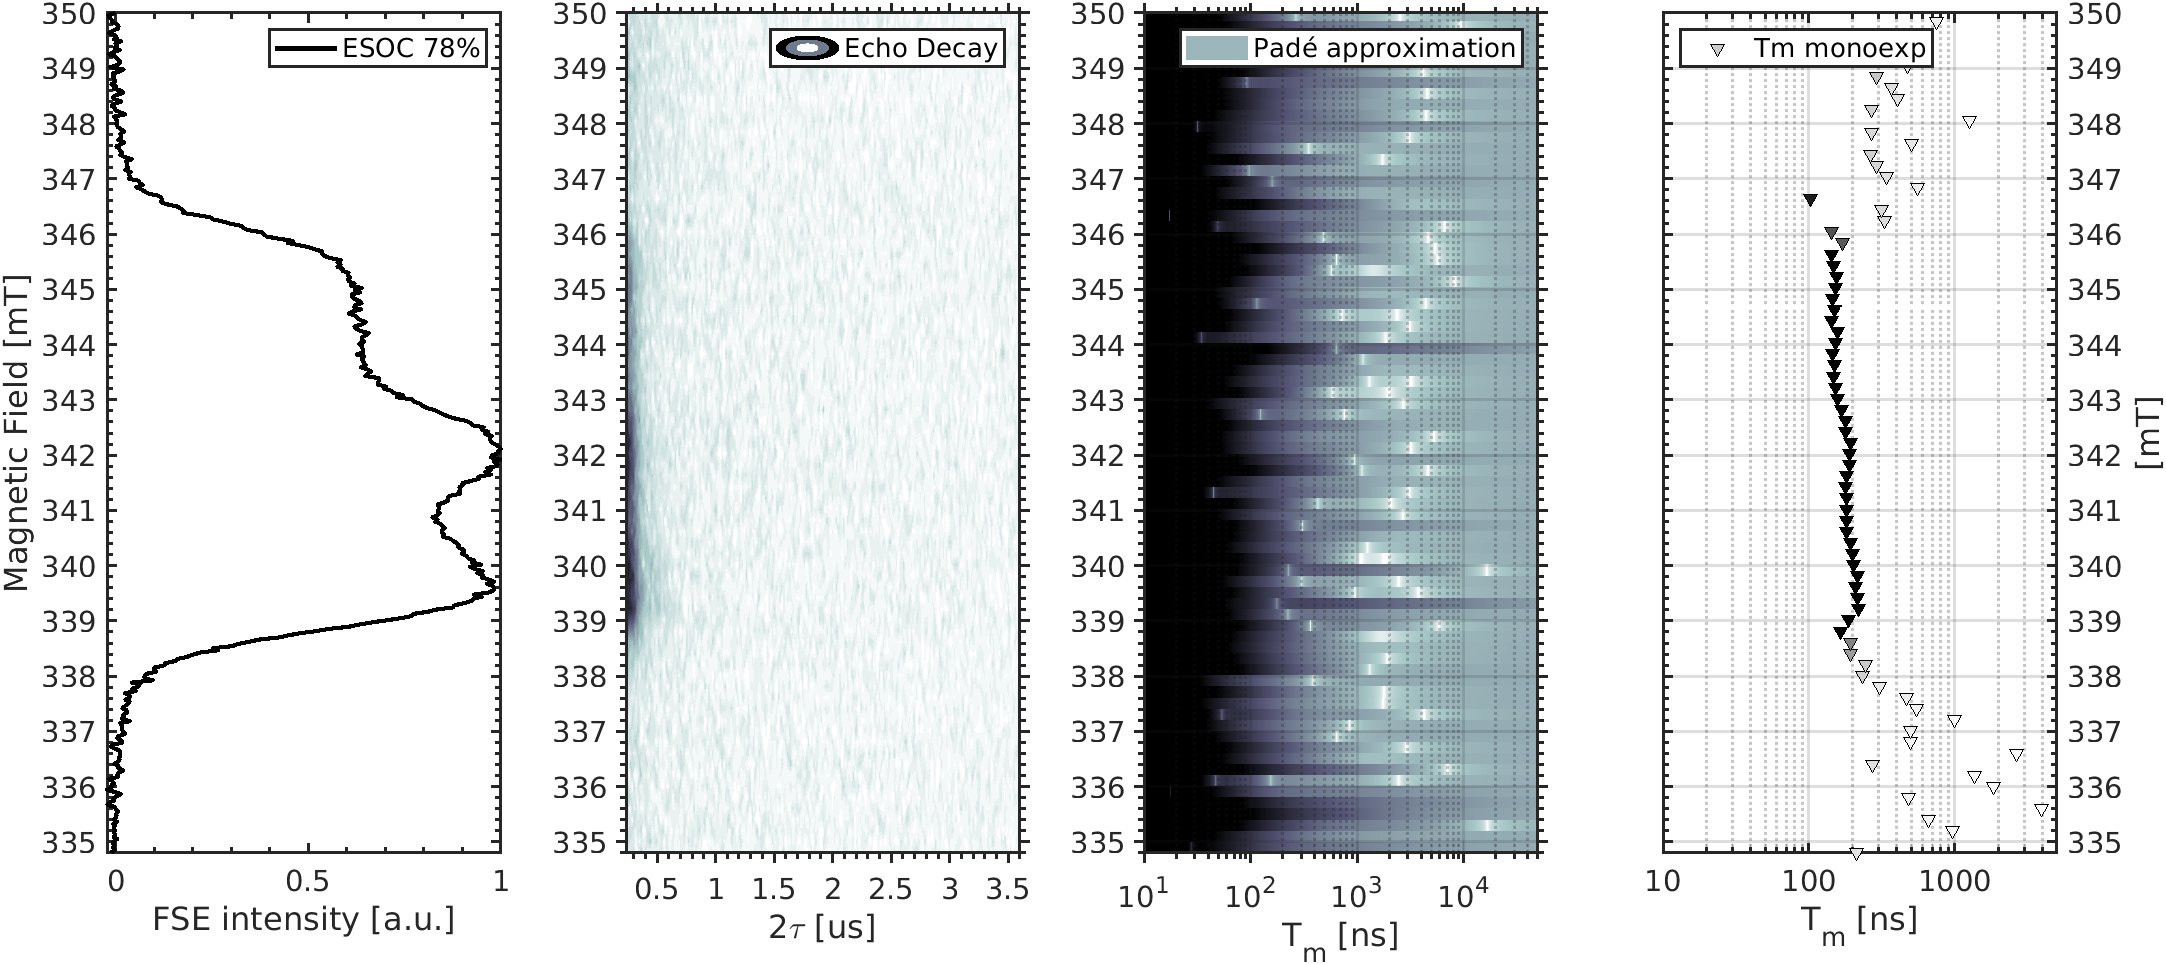
\includegraphics[width=0.5\textwidth]{./pulse/figures/Figure_S12.png}
	\caption{Pad{\'e}-Laplace deconvolution of the field-swept spin echo decay in a pDiTBuS film at 85\%~ESOC. Temperature 5K.}
	\label{fig:Figure_S12}
\end{figure}

\begin{figure}[ht!]
\center
	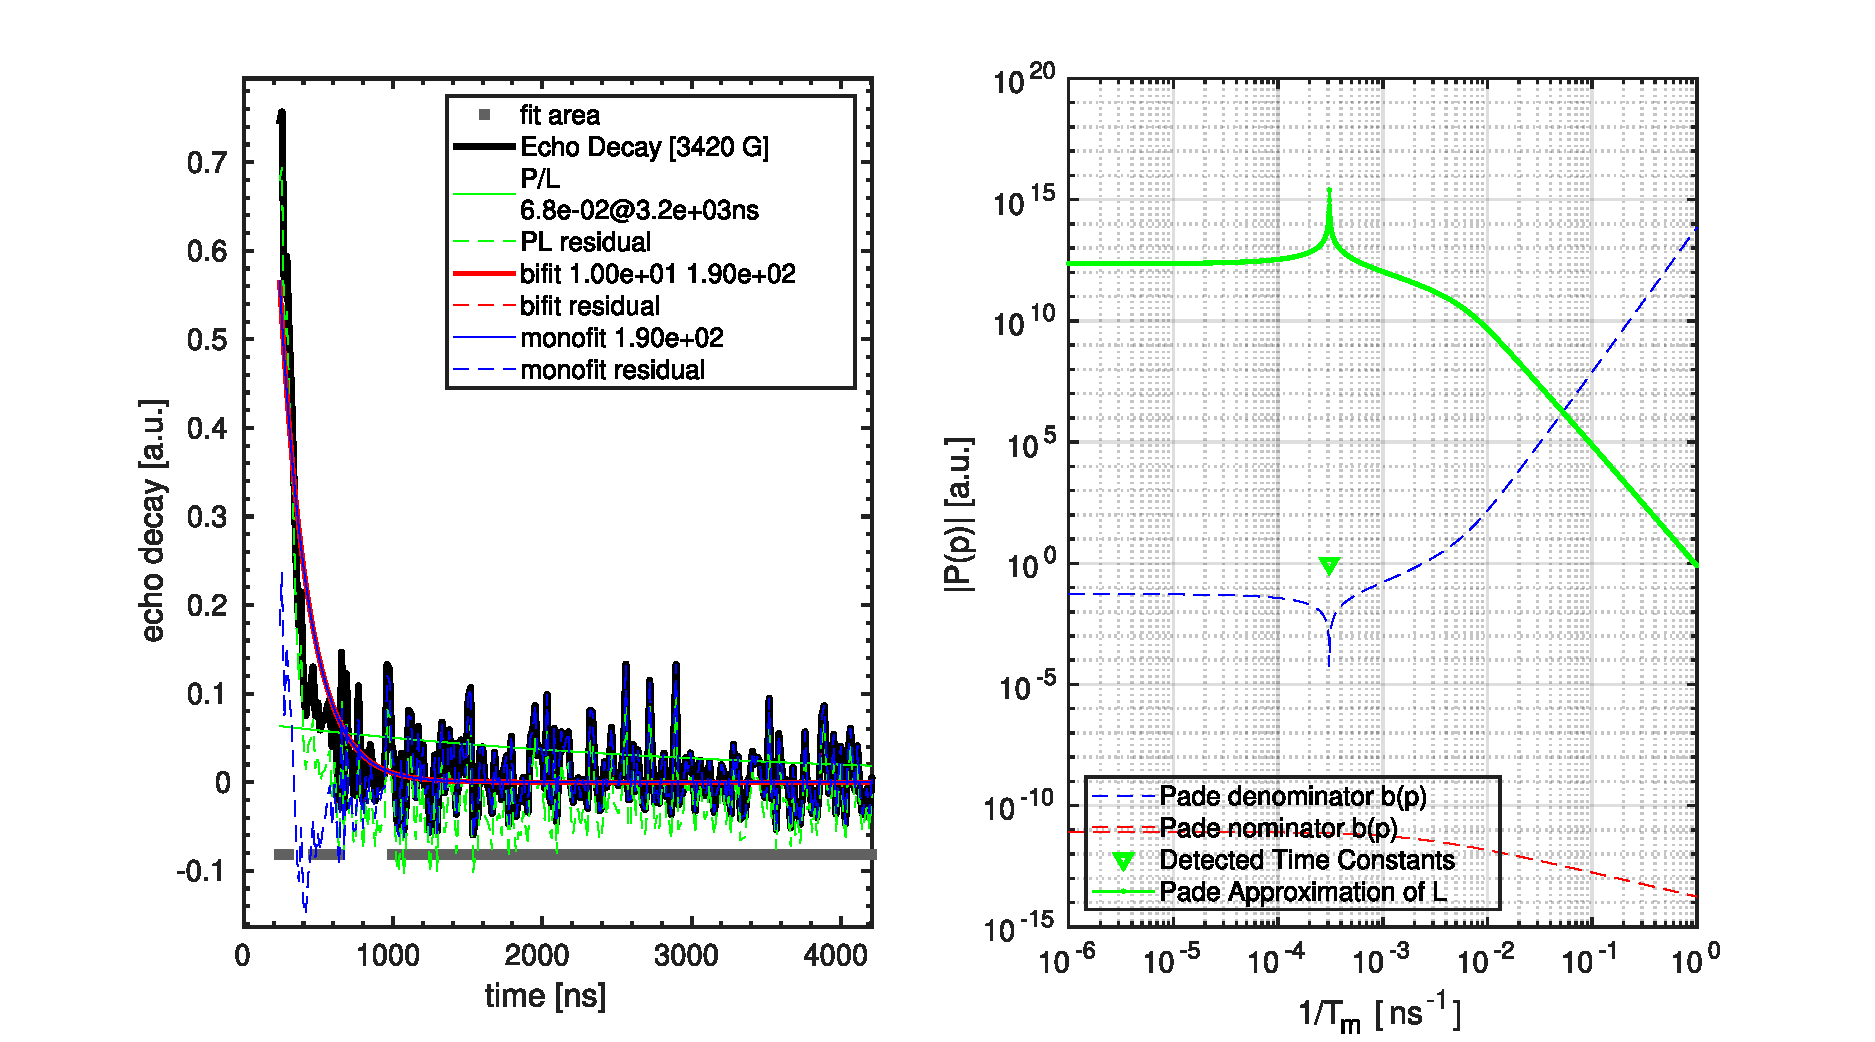
\includegraphics[width=0.5\textwidth]{./pulse/figures/Figure_S13.pdf}
	\caption{Pad{\'e}-Laplace deconvolution, biexponential and monoexponential fits of the spin echo decay in a pDiTBuS film at 85\%~SoC at the $m_I=0$ spectral position. Temperature 5K. Data was fit in the 'fit area' region. ESEEM oscillations were excluded from the data for fit and Pade-Laplace analysis.}
	\label{fig:Figure_S13}
\end{figure}



\newpage
\subsubsection{Inversion Recovery in 50 mM TEMPOL}
\label{esi:pade_laplace_T1}
\begin{figure}[h]
\center
	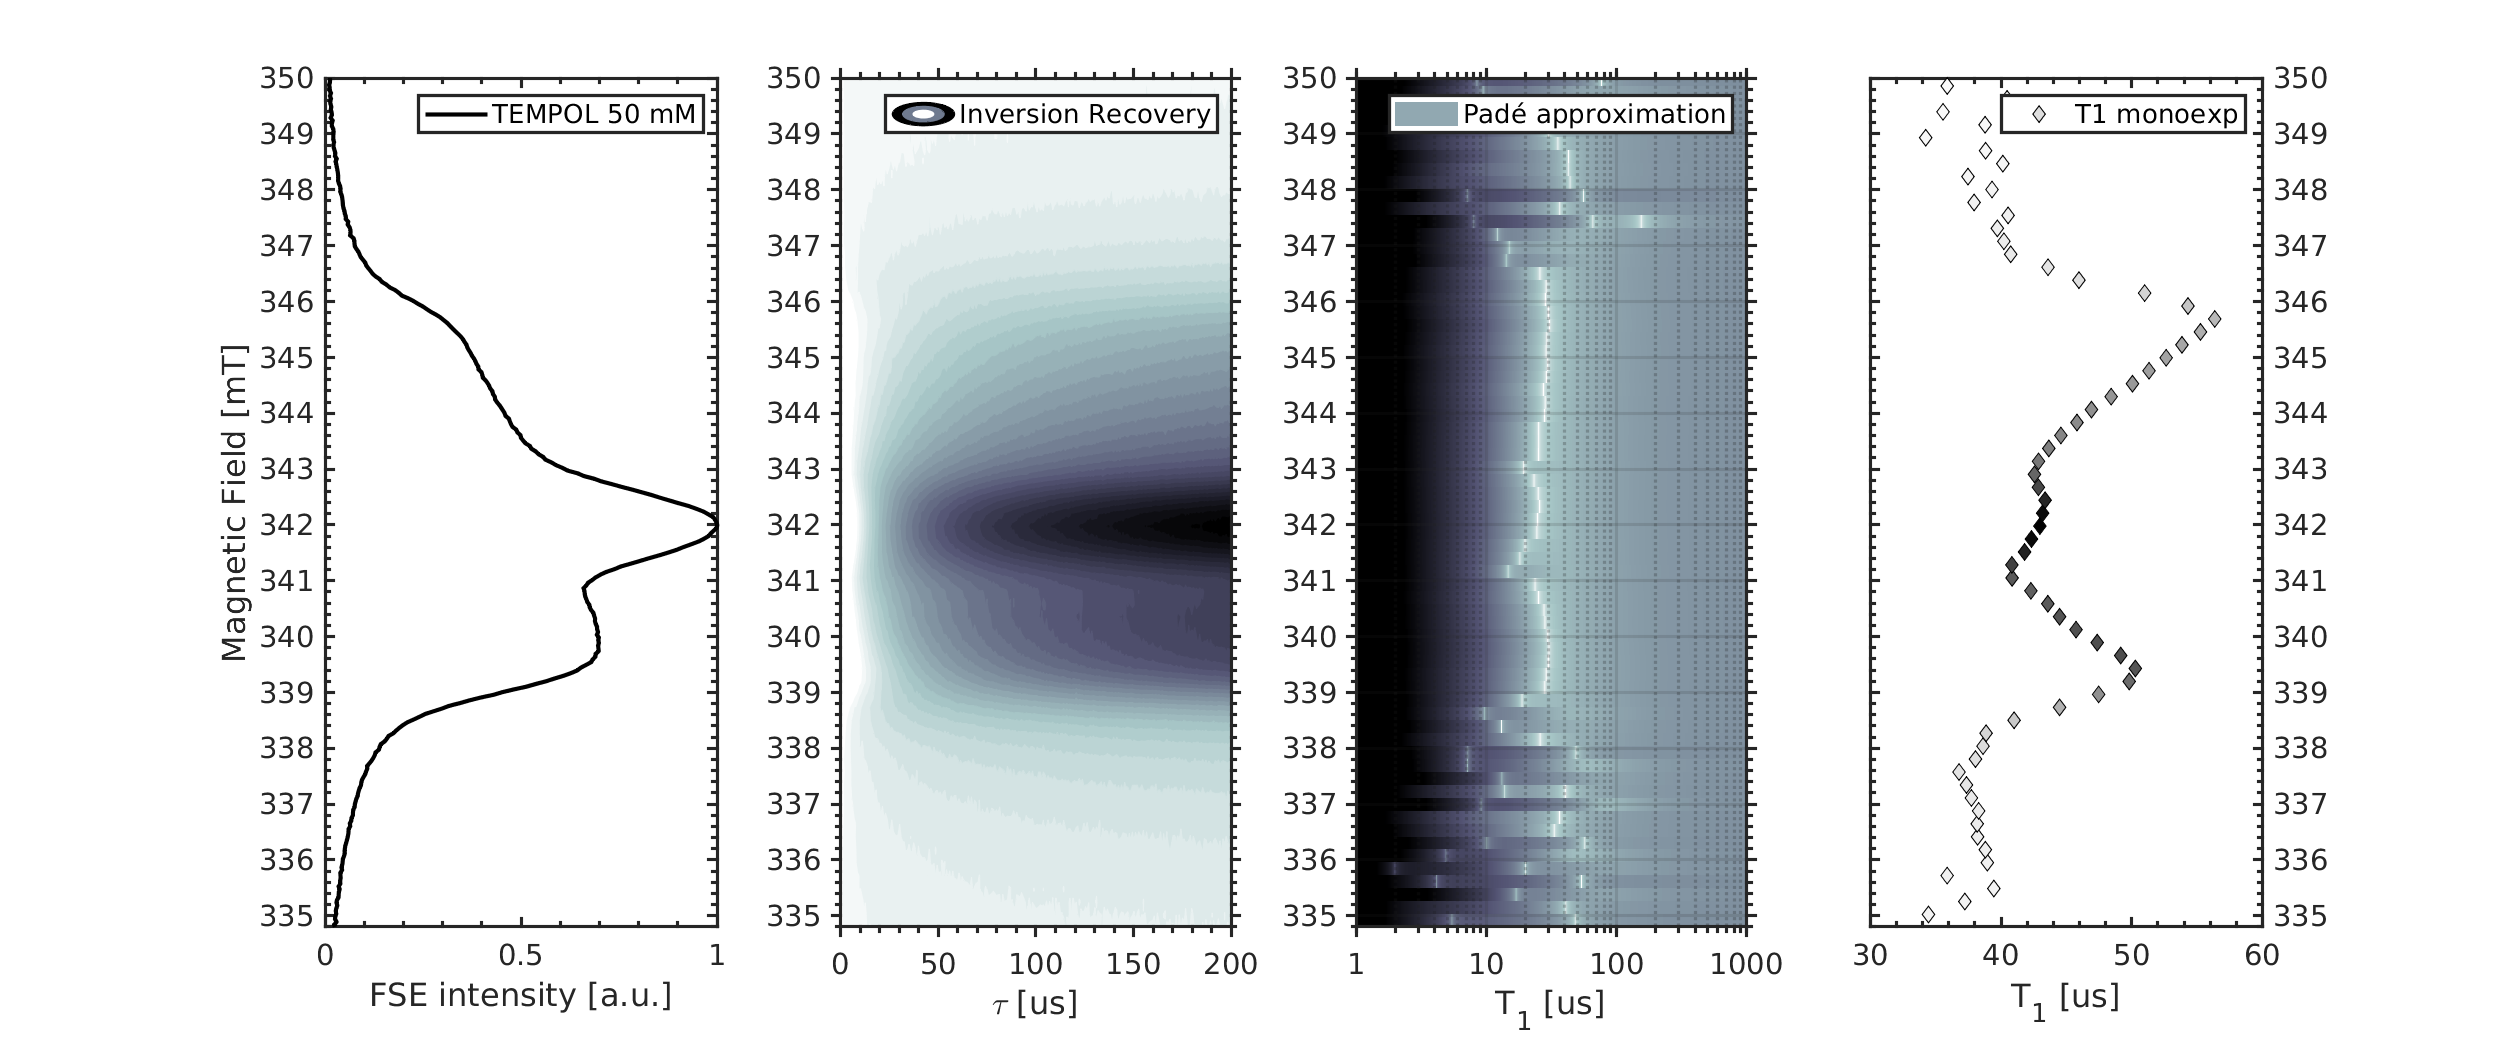
\includegraphics[width=0.5\textwidth]{./pulse/figures/Figure_S14.png}
	\caption{Pad{\'e}-Laplace deconvolution of the field-swept inversion recovery in a frozen 50~\si{\milli\Molar}  solution of TEMPOL in the Dichloromethane:Acetonitrile glass (3:1). Two decay components detected with Pade-Laplace (separated poles in the Pad{\'e}-Laplace approximation, third panel). Biexponential fit (circles for faster component, squares for slower component, right panel). Temperature 5K.}
	\label{fig:Figure_S14}
\end{figure}


\begin{figure}[ht!]
\center
	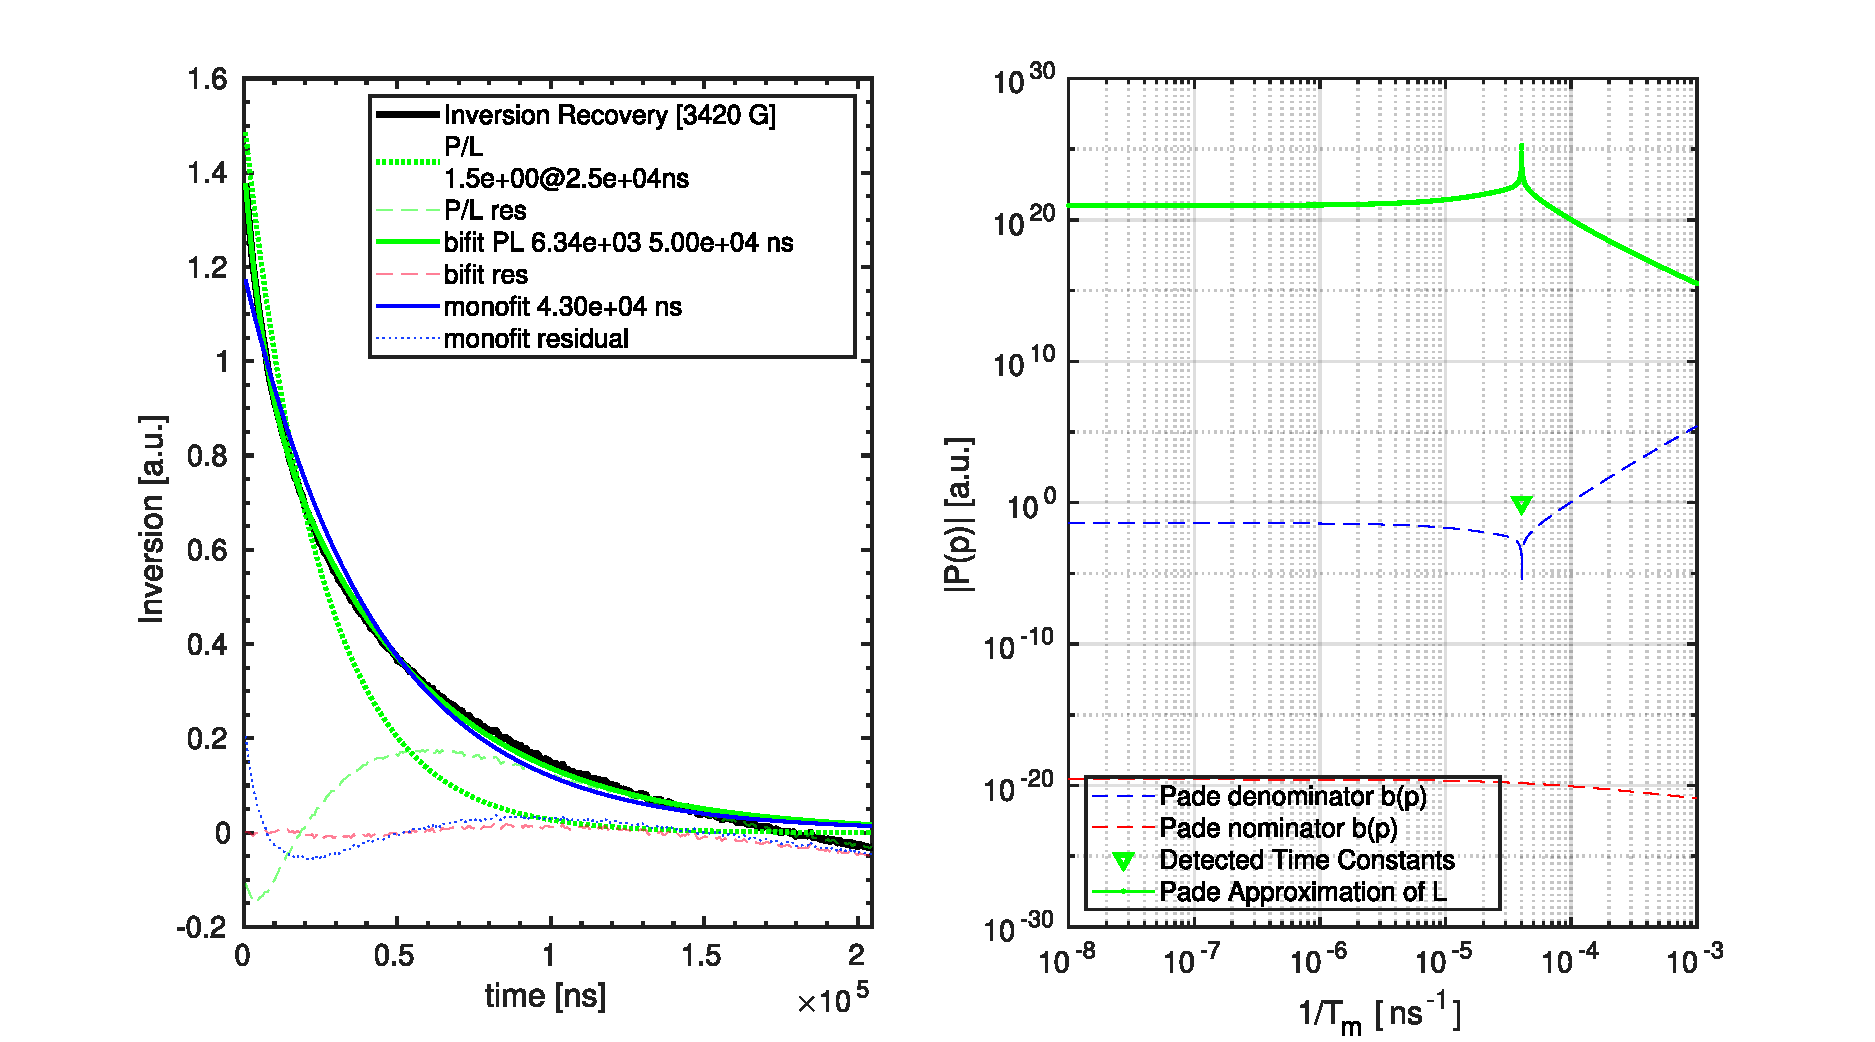
\includegraphics[width=0.5\textwidth]{./pulse/figures/Figure_S15.pdf}
	\caption{Fits of the inversion recovery transient in the frozen 50~\si{\milli\Molar}  TEMPOL solution at the central spectral peak ($m_I=0$, 342~mT). Pad{\'e}-Laplace deconvolution the transient and a biexponential fit. Temperature 5K.}
	\label{fig:Figure_S15}
\end{figure}



\newpage
\subsubsection{Inversion Recovery in DiTBuS 95\% ESOC}
\begin{figure}[h]
\center
	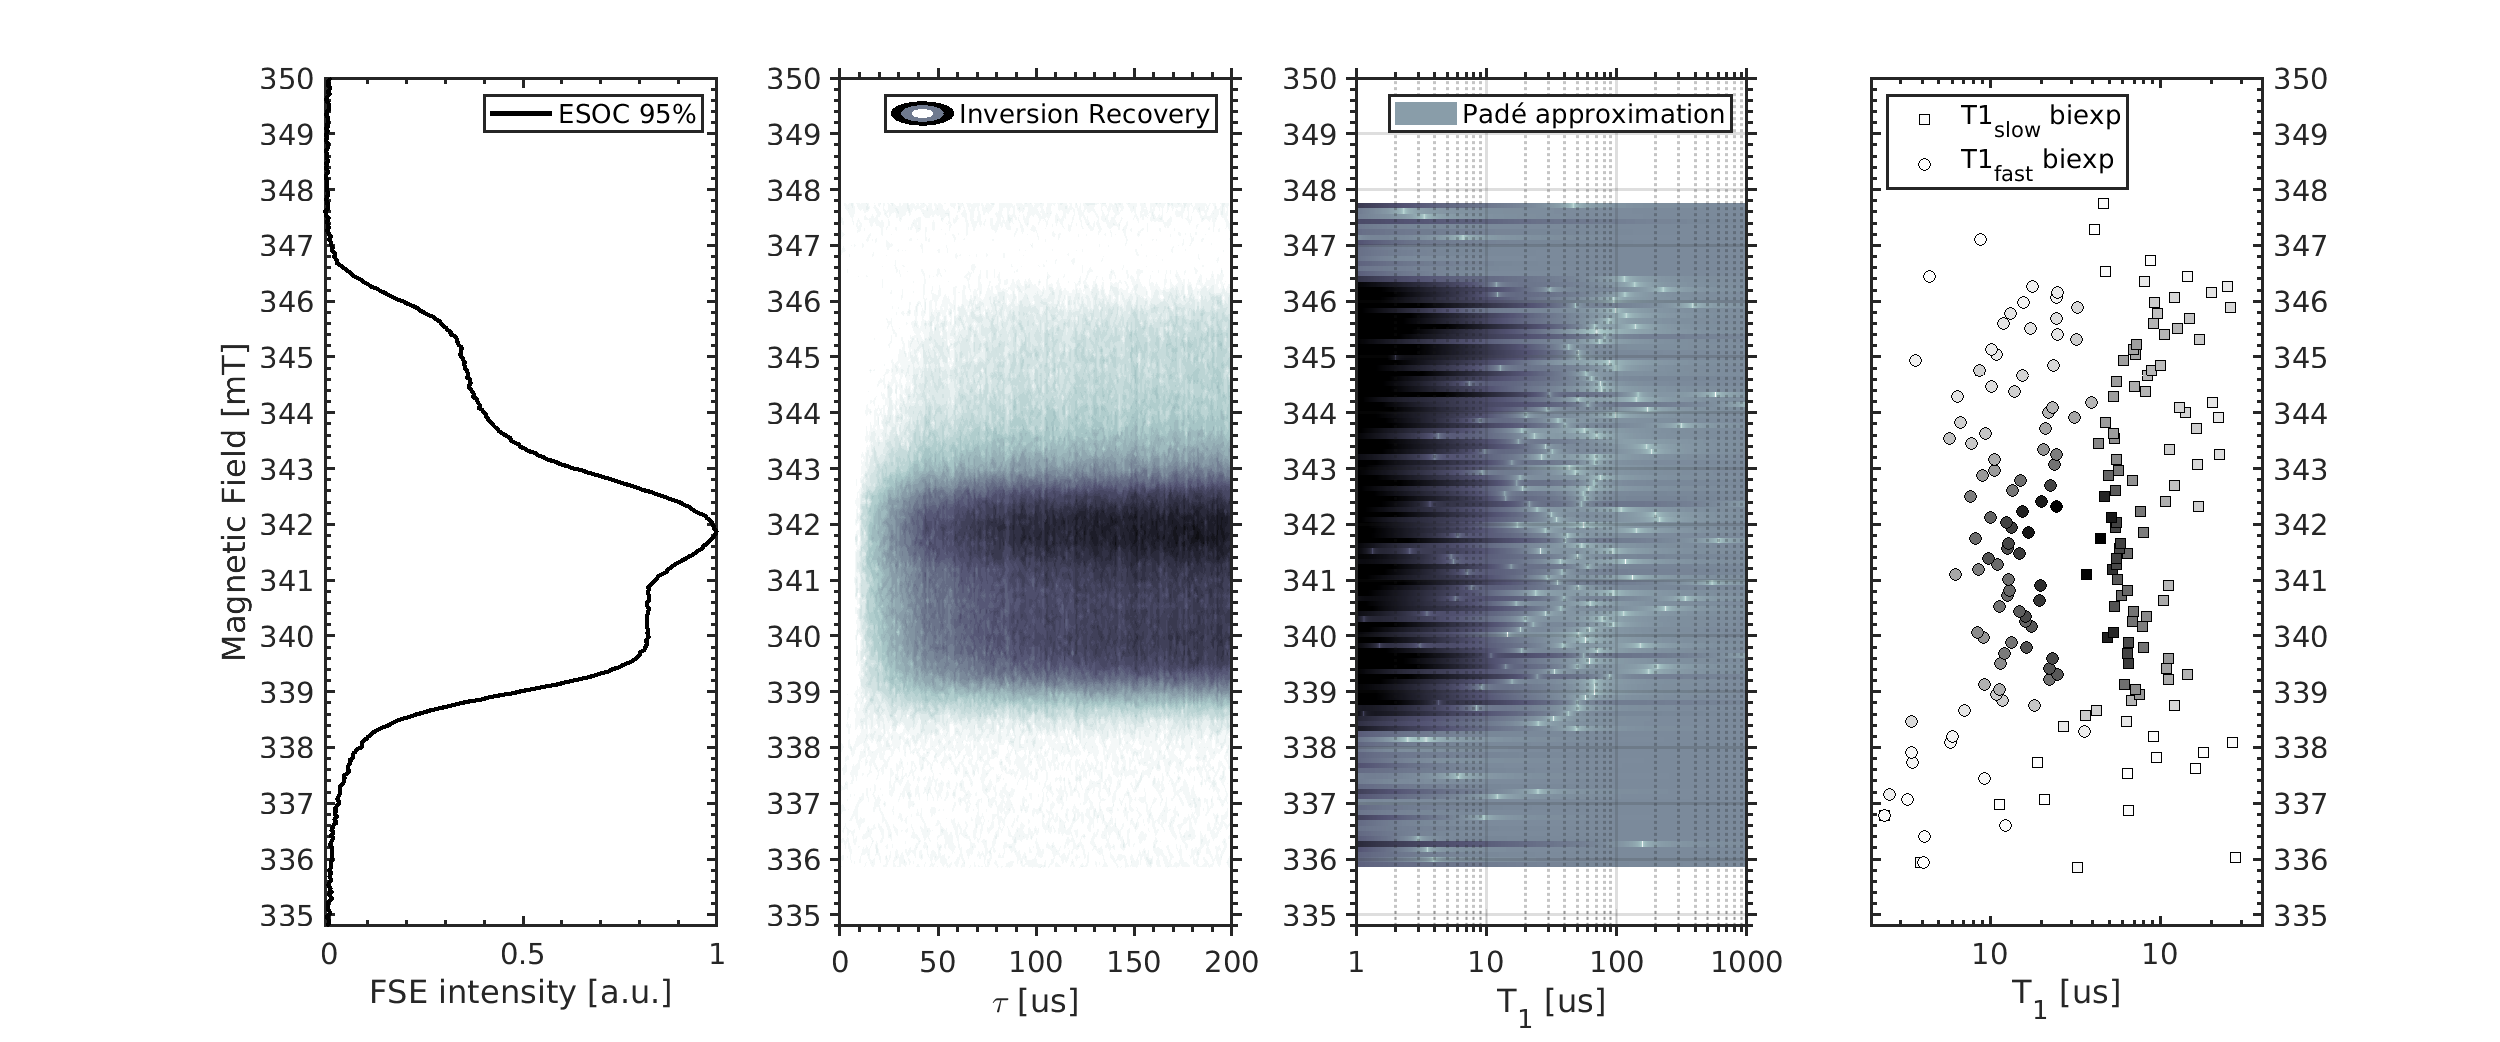
\includegraphics[width=0.5\textwidth]{./pulse/figures/Figure_S16.pdf}
	\caption{Pade-Laplace deconvolution of the field-swept inversion recovery in a pDiTBuS film at 95\%~ESOC. Temperature 5K.}
	\label{fig:Figure_S16}
\end{figure}

\begin{figure}[ht!]
\center
	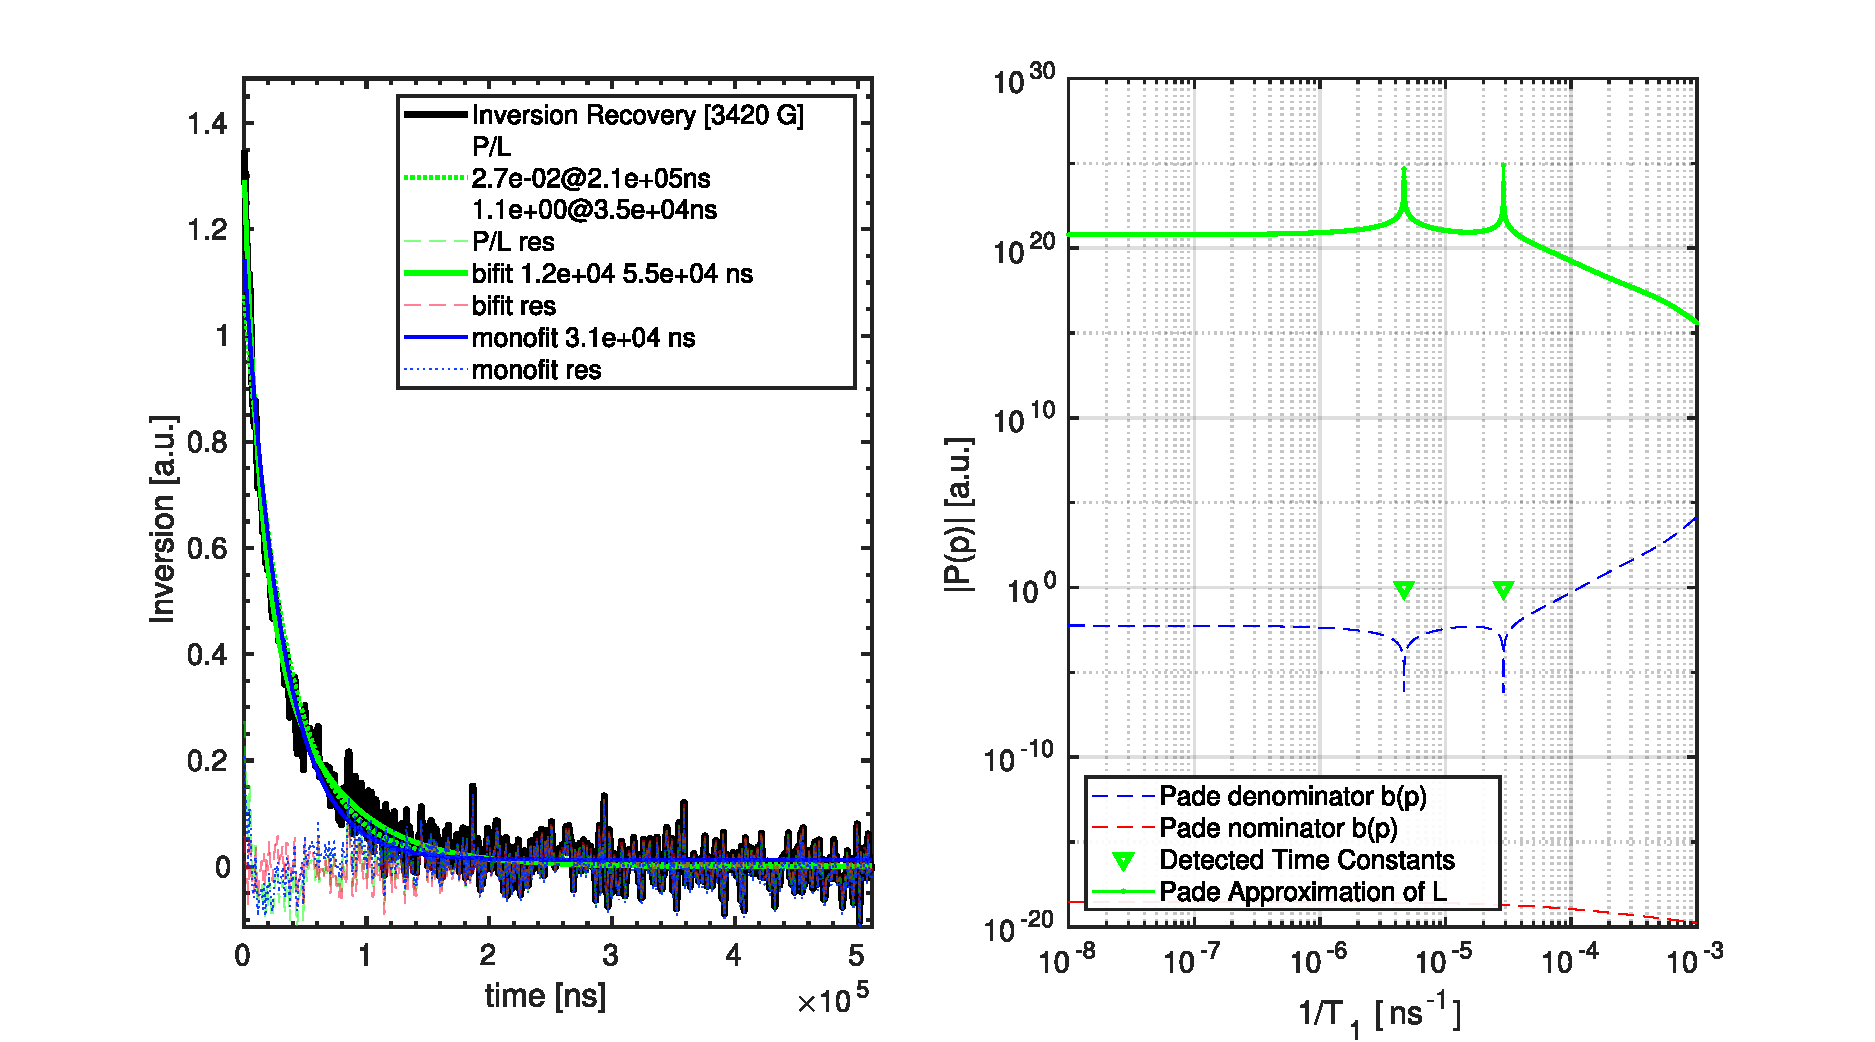
\includegraphics[width=0.5\textwidth]{./pulse/figures/Figure_S17.pdf}
	\caption{Fits of the inversion recovery transient in the 95\% ESOC pDiTBuS film at the central spectral peak ($m_I=0$, 342~mT). Pad{\'e}-Laplace deconvolution the transient and a biexponential fit. Temperature 5K.}
	\label{fig:Figure_S17}
\end{figure}


\newpage
\subsubsection{Inversion Recovery in DiTBuS 85\% ESOC}
\begin{figure}[h]
\center
	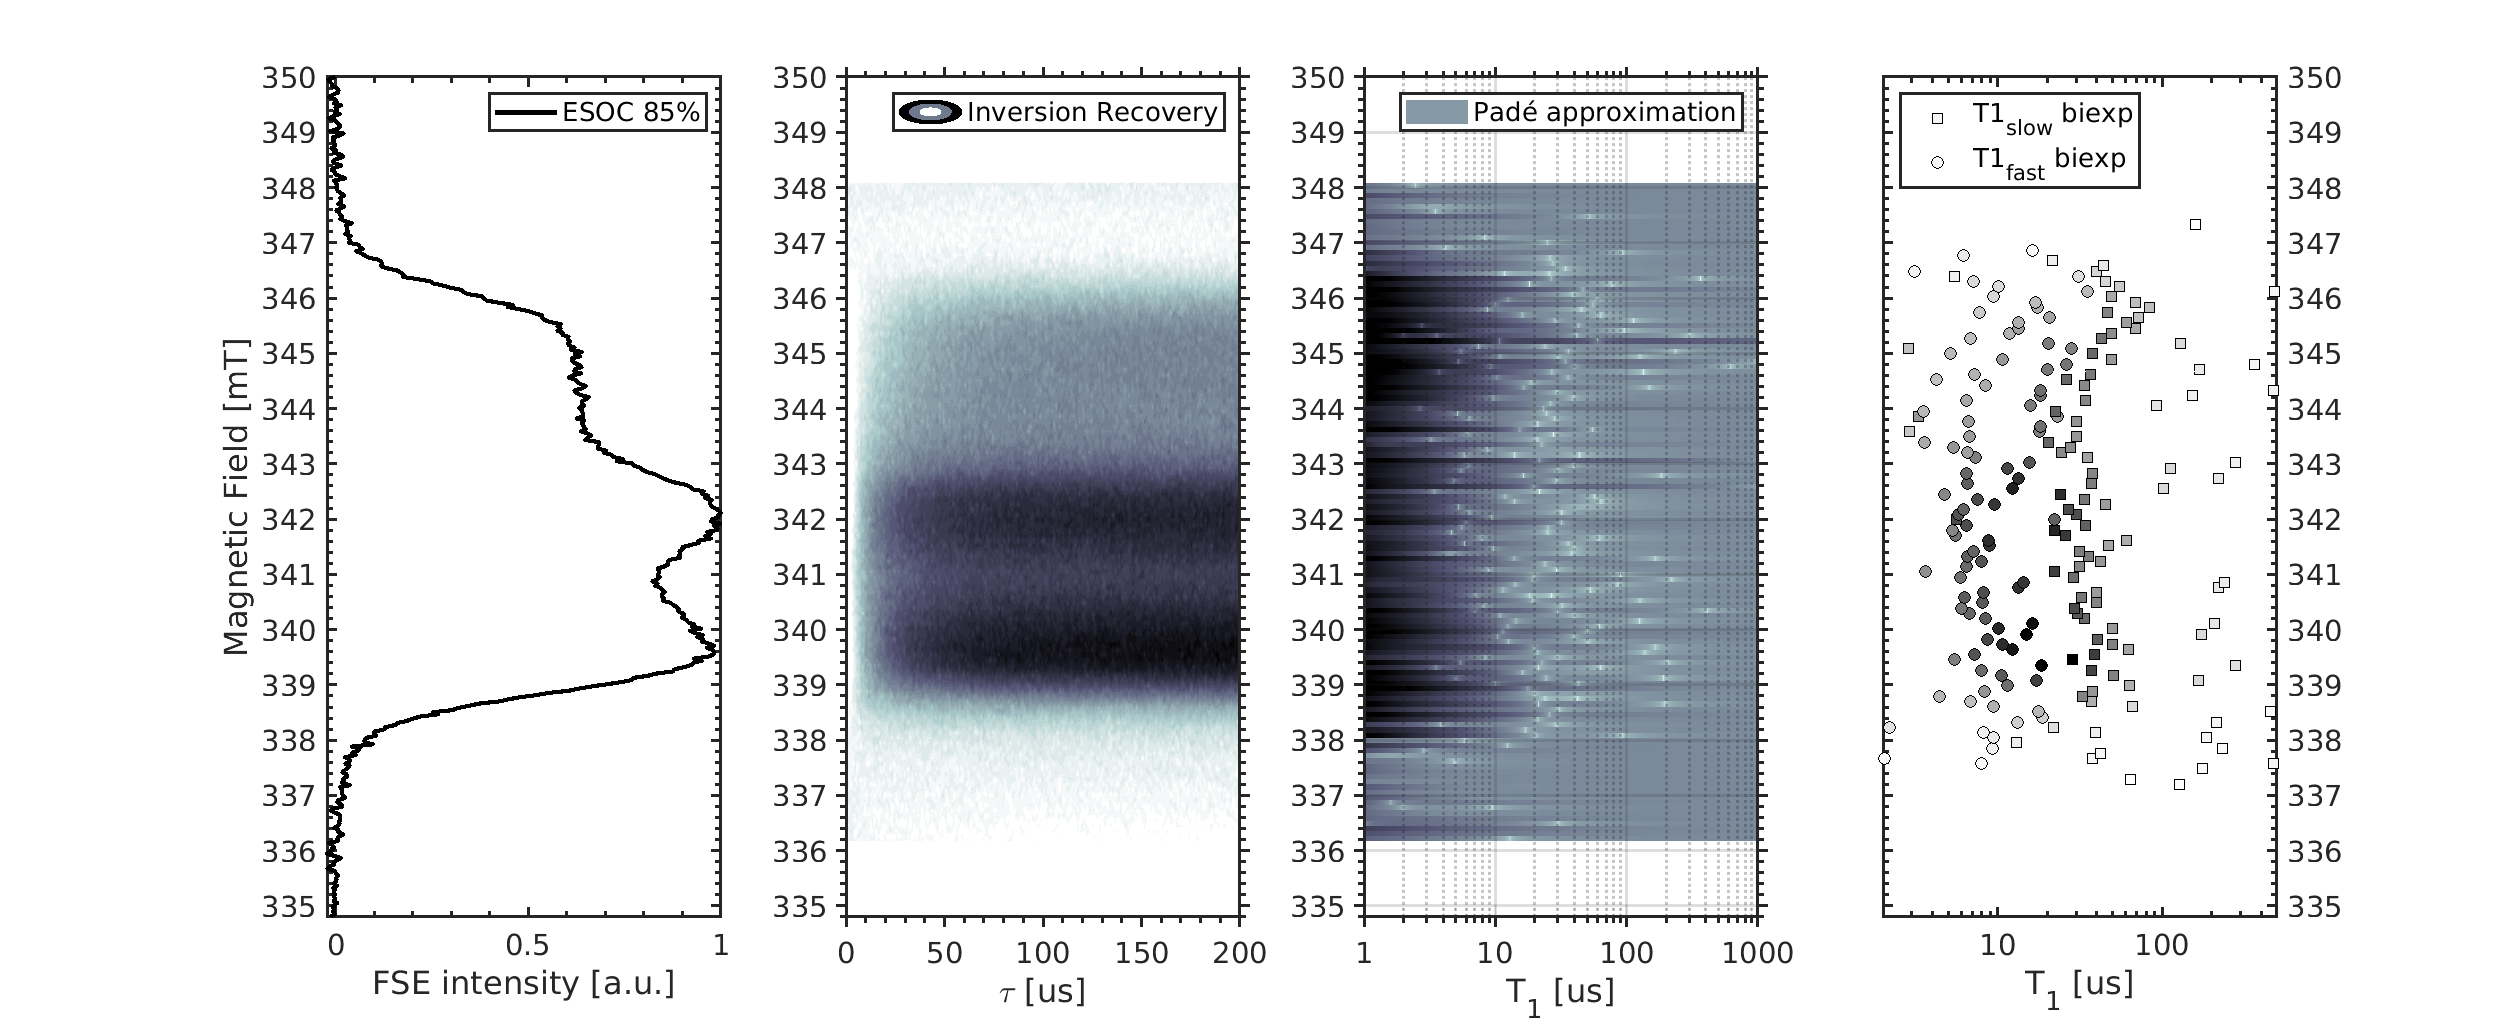
\includegraphics[width=0.5\textwidth]{./pulse/figures/Figure_S18.pdf}
	\caption{Pade-Laplace deconvolution of the field-swept inversion recovery in a pDiTBuS film at 85\%~ESOC. Temperature 5K.}
	\label{fig:Figure_S18}
\end{figure}


\begin{figure}[ht!]
\center
	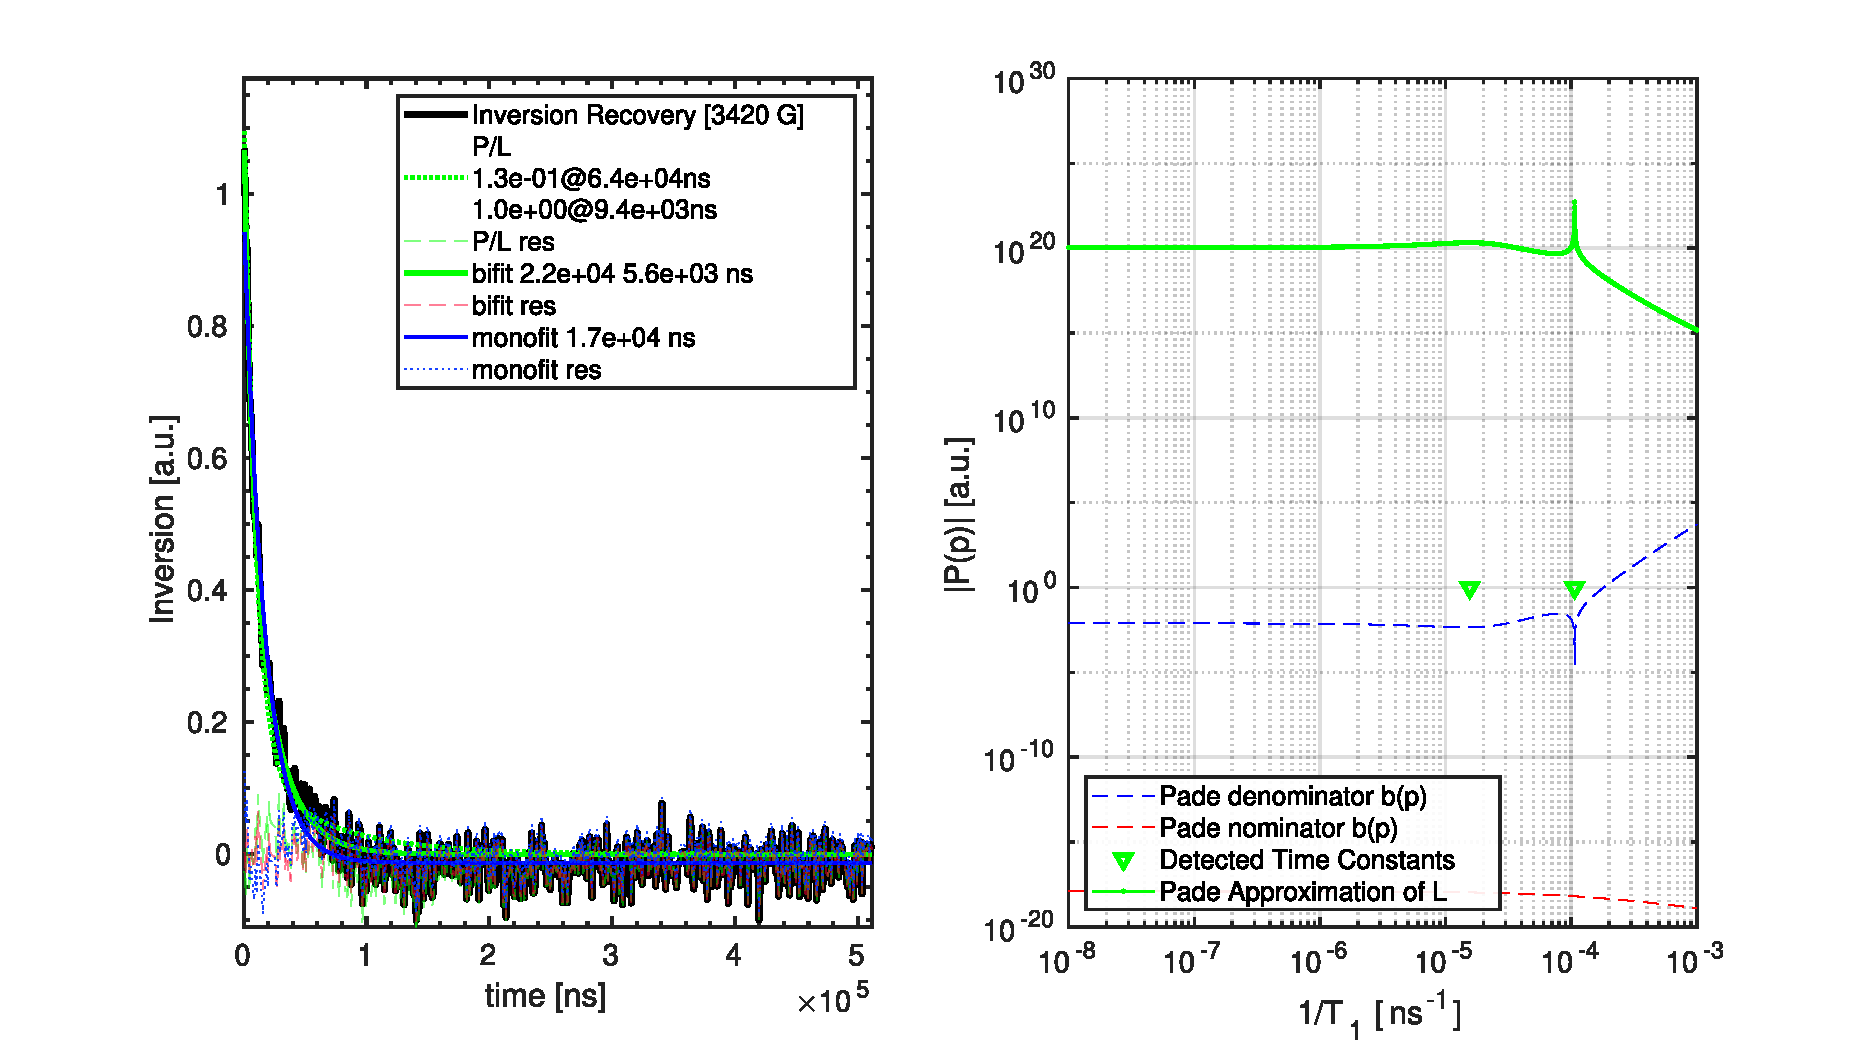
\includegraphics[width=0.5\textwidth]{./pulse/figures/Figure_S19.pdf}
	\caption{Pade-Laplace deconvolution and biexponential fit of the inversion recovery in a pDiTBuS film at 85\%~ESOC at the $m_I=0$ spectral position. Temperature 5K. Data is inverted and scaled before fitting.}
	\label{fig:Figure_S19}
\end{figure}



\subsection{Detection of Domains with Poor Conductivity}
\label{sec:domains_distinction_by_relaxation}

\subsection{Towards Imaging of Spin Concentrations in Battery Electrodes}
The local spin concentrations that are present in an electrode film can be obtained by the time-constant-domain analysis of the echo decay transients, as it was described in \ref{sec:domains_distinction_by_relaxation}. One can extend this characterization technique and obtain a spatially resolved image of the spin concentrations inside the battery electrode by encoding the position at which the sample is excited with a gradient of the magnetic field. A strongly asymmetric ferromagnetic wedge~\cite{SternGerlach1922} can be used to superimpose a gradient of $B_0$ in a chosen direction so one can not only measure the spin concentrations that are present in the electrode, but also to locate the electrochemically inactive domains and to visualize the conductive paths throughout the electrode, analogously to the NMR imaging. The difficulty on the way to apply this visualization technique lies in the large excitation bandwidth of the pulse sequence.
\par
Let the cathode film of width $l$ be oriented along the static magnetic field so that $B_0$ lies in the film plane. Let the $B_0$ be fixed at the maximum intensity of the FSE spectrum, say, $B_0 = B_0^{res}=342$~mT. Let $B_0$ be homogeneous within the film length, which is normally the case for the EPR resonator. Let the film contain a distribution of spin concentrations within its length $C_{min}<C(z)<C_{max}$. With the homogeneous $B_0$, the microwave pulse will excite the entire film length and the spin echo signal will contain spin echoes from all length elements of the film, that correspond to all $C(z)$. The inversion recovery transient will contain the time constants from all length elements of the film $T_1(z)$. With the Pad{\'e}-Laplace analysis one recovers the distribution of the concentrations within the film $C_i$, but since the $B_0$ is homogeneous, the information on the position $z_i$ at which the domains are located, is lost. 
\par
Let now the $B_0$ to be linearly increasing from $B_0(z=-l/2) = B_0^{res}-\Delta B_0$ at one side of the film to $B_0(z=l/2)=B_0^{res}+ \Delta B_0$ by the other side of the film, so that for a given length element $dl$ the inhomogeneity of $B_0$ is $dB/dl = \frac{B(z=l/2)-B(z=-l/2)}{l}$. In the center of the film (at $z=0$) the $B_0$ is resonant and the spin echo signal will be generated, while from the other positions of the film the magnetic field will be non-resonant and no spin echo signal will be generated. Let the width of the EPR spectrum be $\Delta B_{FWHM}=8$~mT and that to define the probed length element $\Delta l$ with the given $B_0$ gradient. $\frac{\Delta B_{FWHM}}{\Delta l} = \frac{B(z=l/2)-B(z=-l/2)}{l}$, so the spatial resolution is 

\begin{equation}
\label{eq:ERI_resolution}
\frac{\Delta l}{l} = \frac{\Delta B_{FWHM}}{B(z=l/2)-B(z=-l/2)}
\end{equation}

With the spectral width of $\Delta B_{FWHM}\leq8$~mT and the film width of $l\leq3\times10^{-1}$~cm to get 
256 points per film length one needs a $B_0$ gradient of $dB/dl \geq 256*8/0.3 \geq 6.8$~[T/cm] which is a realistic value for a typical Stern-Gerlach apparatus~\cite{SternGerlach1922,Liang_2020}. 
